\chapter{Problem Formulation and Methodology (Dust JCA)} \label{ch:methods}
    This chapter defines the methodology used throughout this work. It does not document every implementation detail. The goal is to state the scientific workflow clearly enough for the reader to see what is evaluated, on what evidence, under which physical assumptions, and with which mission-level semantics. The chapter moves from the overall architecture of the study to the detailed treatment of transfer solving, dust mass accounting, uncertainty propagation, constellation encoding, and optimizer comparison.

    Candidate constellations are evaluated on the catalogue-conditioned natural conjunction bank; each scenario is screened through transfer feasibility, dust-delivery physics, and uncertainty-aware mass accounting; and the resulting outcomes are aggregated into mission-level reliability and resource metrics for optimizer comparison. The remaining sections unpack each stage of that workflow.

    \begin{quote}
    \textbf{Held pending independent model authority.} Current quantitative attainment is held, and the descriptive replication policy prohibits global or per-family optimizer-winner claims. Atmosphere decision D1 selects the \gls{jb2008} in its compiled fitted-kernel form; the versioned synthetic thermosphere proxy is not used, and drag-qualified claims are conditioned on the sealed driver scenario described in \cref{ss:propagation}. The probability-qualified released-mass claim remains held pending immutable-receipt sensitivity and exact-commit/archive validation; D2 now defines finite physical-grain mass probability, while historical effective-packet arithmetic is non-authoritative. Momentum enhancement and operational risk-reduction interpretations remain parametric or out of scope until their respective authority gates close.
    \end{quote}

    \noindent\textbf{ECF concept traceability and limits.} The \emph{Fitzgerald ECF 23 Summary} is concept authority for coupling hazardous-event access, transfer opportunity, dust interception, and nondominated architecture tradeoffs; it is not numerical-solver or validation authority. This dissertation's public-catalogue-conditioned natural conjunction bank differs from the literal proposal pseudocatalog and must be identified as such in any cross-document claim. The production baseline permits a minimum lead time of \SI{6}{h}, whereas the concept summary describes roughly half-day timing; a matched \SI{6}{h}/\SI{12}{h} sensitivity is required before any proposal-faithful timing claim. Two configured release fractions and a solved release-control vector provide partial cloud adaptability, but fixed grain and dispersion parameters mean the study does not jointly optimize all cloud designs described in the concept. Each modeled unsafe event is one debris pair; a breakup-cloud multi-fragment event is outside scope. Response time and plane count remain design metadata or constraints, not independent publication-front axes, whose physical coordinates are executed maneuver and released mass. Finally, trajectory feasibility and architecture analysis provide no flight-hardware or technology-readiness-level validation.

\section{Dust JCA Problem Formulation} \label{se:problem_formulation}
    In operational terms, the task is to evaluate deployer-constellation designs intended to retire unsafe conjunction opportunities under strict physics and timing constraints while minimizing mission resource demand. Let \gls{sym:x} denote a candidate constellation design, and let \gls{sym:omegaunsafe} denote the catalogue-conditioned natural conjunction bank.

    Evaluating \gls{sym:x} over \gls{sym:omegaunsafe} yields:
    \begin{itemize}[leftmargin=*]
        \item event-level transfer/intercept feasibility outcomes under active solver limits;
        \item event-level released dust mass requirements from encounter-plane coverage conversion;
        \item event-level deterministic intercepted-mass validity under the active strict event-feasibility policy;
        \item mission-level reliability/resource summaries for optimization and reporting.
    \end{itemize}

    The final mission objective pair comprises \gls{sym:j1} for deployer maneuver burden and \gls{sym:j2} for released dust mass burden. Their raw inputs remain distinct and are reconstructed from event-level nondominated fronts. For a configured coverage fraction \(q\), the canonical objective is the nondominated set of resource boxes \((d,M)\) that can service at least \(k=\lceil qN\rceil\) members of the fixed \(N\)-event bank with per-event executed maneuver no greater than \(d\) and released dust mass no greater than \(M\). The production bank has \(N=64\) and \(q=0.9\), hence \(k=58\). Beta/HPD state is an operational search controller only; canonical coverage is an exact finite-bank count. Deterministic intercepted-mass sufficiency is not optimized as a soft preference; it remains a strict event-level acceptance gate.

\section{Mission Overview} \label{se:mission}
    The end-to-end workflow begins with a reusable catalogue-conditioned natural conjunction bank. A candidate constellation is then decoded into deployer orbits, screened against shared scenario evidence, and passed through the transfer solver and dust-mass logic. Event-level outcomes are then aggregated into mission-level reliability and resource scores so that optimizer comparisons rest on the same evidence and the same operational semantics.

    Under routine cataloging and screening operations, endogenous debris threats are often identifiable days before conjunction. Let \(P_c(t)\) denote the current estimate of collision probability for a predicted conjunction at epoch \(t_0\). Following initial detection near \(t_0-7~\mathrm{days}\), an automated monitor ingests refined tracking updates and recomputes \(P_c\) as state uncertainties contract.

    A notional two-threshold triage policy helps balance responsiveness against unnecessary actions: (i) an advisory level, for example \(P_c \ge P_c^\mathrm{adv}\), which triggers active tasking and reachability checks; and (ii) a commit level, for example \(P_c \ge P_c^\mathrm{com}\), above which the system prepares to execute remediation. In baseline simulations, execution is ultimately driven by minimum lead-time and feasibility constraints, so the \(\SI{1}{\%}\) commit level is used here as timing context. If by \(t_0-48~\mathrm{h}\) the updated probability remains above \(P_c^\mathrm{com}\), the system commits subject to required lead time \(t_\ell \ge t_\ell^\star\) between dust intercept and closest approach. This lead time keeps the required effective \(\Delta V\) in a feasible range and leaves margin for post-intercept state confirmation.

    For each conjunction pair, one object is designated as the primary target, that is, the object to be nudged. The decision balances expected risk reduction, reachable geometry, and the operational burden of delivering the intervention. A deployer is then selected through a staged transfer workflow: candidate pairs are screened with fast heuristics, phasing and multi-revolution Lambert branches generate a transfer Pareto set, and every replay-verified transfer retained for canonical evaluation is crossed with every configured release fraction. The catalogue intercept epoch is fixed; final evaluation does not retime it or collapse the transfer set to one preselected candidate.

    For the short horizons relevant to \gls{jca} (hours to two days), simulations allocate fidelity by body role and epoch. Catalogue scenario construction uses the tractable analytical/\(J_2\)-class lane. Lambert and \(J_2\) machinery provide transfer seeds, while production transfer-front candidate generation/verification and canonical replay require strict HF authority; the \(E_0\rightarrow L\) transfer body uses a gravity-only HF context. The canister coast and released-dust flight are separate HF arcs with separate immutable ballistic tuples. The dust arc uses fixed \(5\times5\) spherical-harmonic gravity, drag, \gls{srp}, Sun, and Moon terms with interpolated ephemerides; its configured physical window is at most two hours. \Gls{sgp} is used only to propagate the pinned \gls{omm} captures to the common source anchor; no \gls{tle} ingestion path exists.

    Dust deployment is adaptive to the remediation task through the solved release-control vector, configured release fraction, and propagated uncertainty state. Across all modes, the mission planner enforces a minimum lead time between dust intercept and conjunction so that the induced orbital change meaningfully separates the target from the conjunction funnel before closest approach.

    The modeled canister is a trajectory-reference body, not a hardware sizing model. It uses the fixed spherical-equivalent tuple \(A/m=0.01~\si{\metre\squared\per\kilogram}\), \(C_D=2.2\), and \(C_R=1.3\) on the HF coast from transfer burn epoch \(L\) to release epoch \(R\). No mesh, dry mass, payload capacity, or dust-mass feedback is modeled. At \(R\), one solved ECI release-control vector is applied exactly once; the released dust then starts from that post-control state. Direct release, dust--spacecraft recontact scoring, hardware feasibility, and operational re-tasking logic are outside the implemented study workflow.

    Maneuver \(\Delta V\) is therefore an executed kinematic impulse burden under an external-impulse assumption. The model does not convert \(\Delta V\) into propellant, wet mass, launch mass, or monetary cost. This deliberate ``resources unconstrained except maneuver and dust'' scope asks how much impulse and dust the concept requires before imposing a particular spacecraft or budget architecture.

    After dust-primary intercept, a bounded verify-and-guard concept would update the primary state, rescreen the former conjunction, check nearby protected objects, and assess dust dilution or decay. The implemented study records these as safeguards and limitations; it does not simulate closed-loop tracking, a second release, deployer trim, or fallback escalation.

    For clarity, the nominal response timeline is:
    \begin{itemize}[leftmargin=1.25em]
        \item \(\mathbf{t_0 - 7\,\mathrm{d}}\): Detection; begin intensive monitoring and advisory tasking.
        \item \(\mathbf{t_0 - 72\,\mathrm{h}}\): Candidate deployers scored on reachability and expected \(P_c\) reduction; phasing plans generated.
        \item \(\mathbf{t_0 - 48\,\mathrm{h}}\): Commit if \(P_c \ge P_c^\mathrm{com}\) under refined tracking. Lock fixed dust model, release-fraction grid, and control/coverage requirements.
        \item \(\mathbf{t_0 - 24\,\mathrm{h}}\): Refine the selected intercept geometry and verify guardrails under the latest tracking update.
        \item \(\mathbf{t_0 - t_\ell}\): Eject the modeled canister and execute dust release to achieve intercept. Begin verify-and-guard assessment.
        \item \(\mathbf{t_0}\): Former conjunction epoch; screen for residual risk and for secondary hazardous geometries created by the intervention.
    \end{itemize}

\begin{figure}[H]
        \centering
        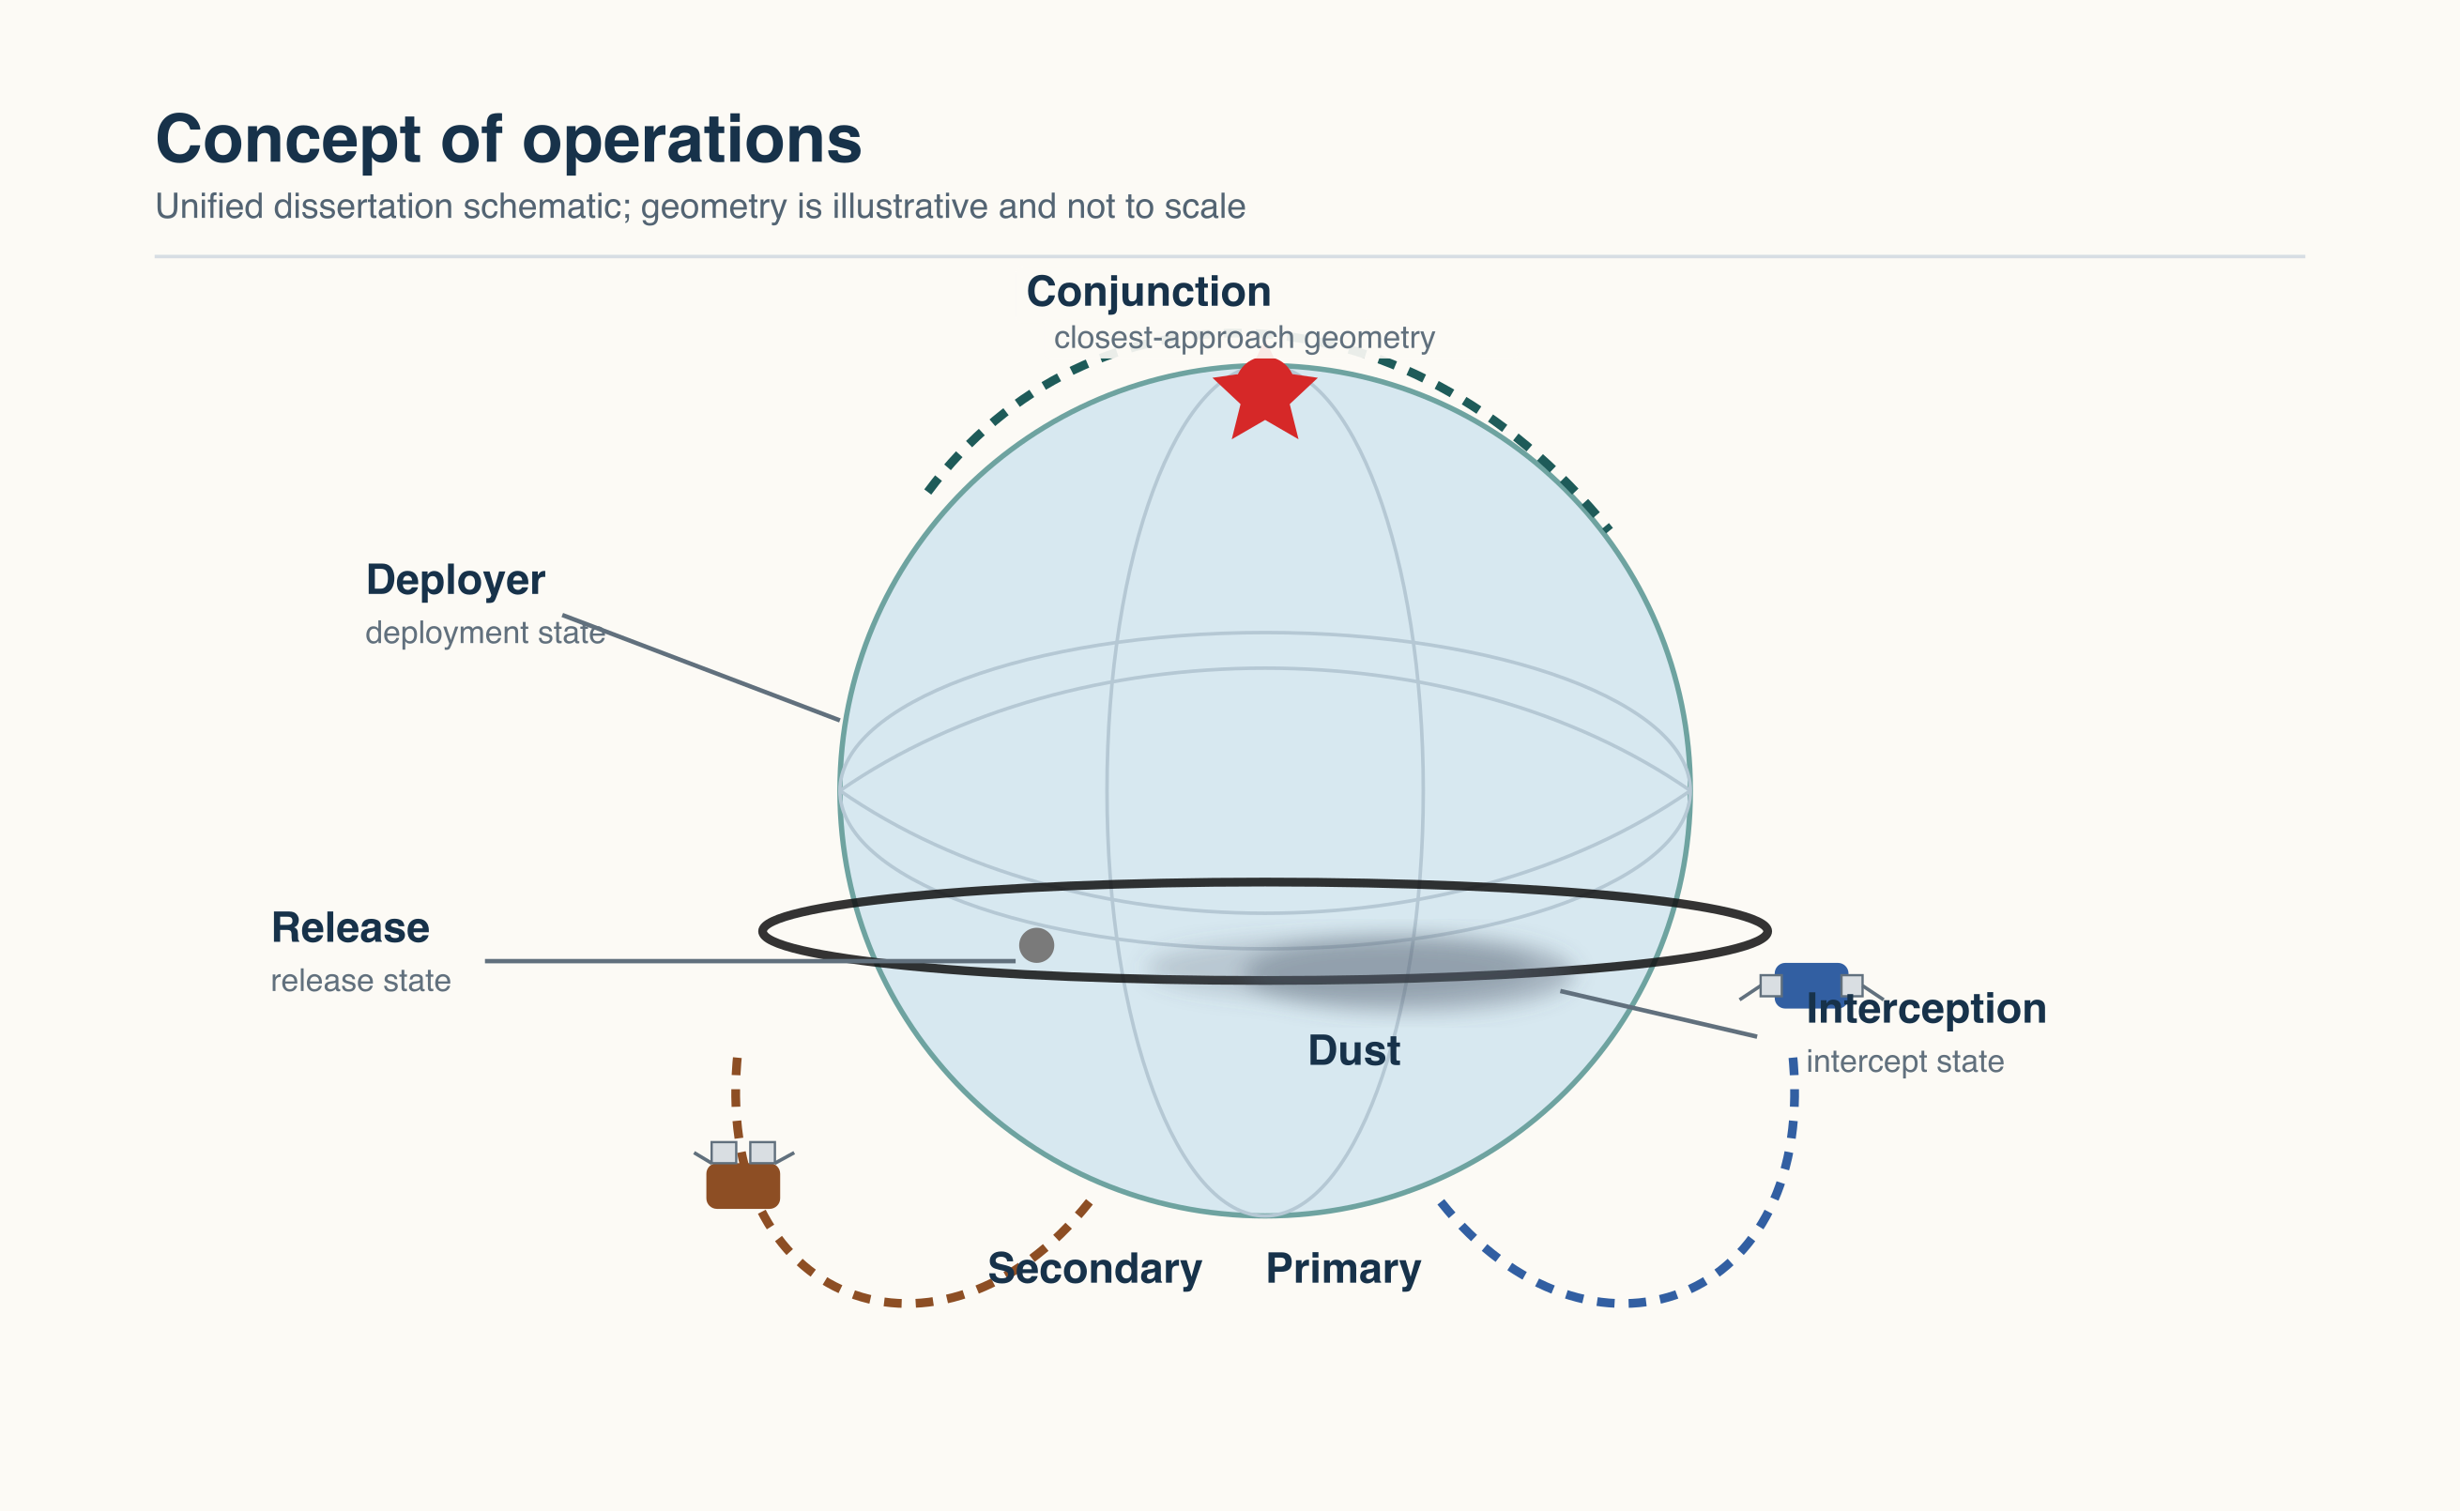
\includegraphics[width=0.96\linewidth]{figs/conops.png}
        \caption[Concept of operations for dust-based JCA]{Concept of operations schematic for dust-based JCA. Representative deployer trajectories stage a dust release ahead of closest approach so the cloud intercepts the target before conjunction and imparts a small separating perturbation. Geometry is illustrative and not to scale.}
        \label{fig:conops}
    \end{figure}

    \begin{table}[htb]
        \centering
        \caption[Operational triage thresholds]{Operational triage thresholds and timing parameters (illustrative policy context; numerical defaults are specified in the run configuration as detailed in \cref{se:constraints,se:optsetup}).}
        \begin{tabularx}{0.92\linewidth}{@{}L{0.19\linewidth}Y L{0.28\linewidth}@{}}
            \toprule
            Parameter & Meaning & Baseline value \\
            \midrule
            $P_c^{\mathrm{adv}}$ & Advisory threshold to begin tasking & $10^{-4}$ (representative; adjusted per scenario) \\
            $P_c^{\mathrm{com}}$ & Commit threshold for remediation & $0.01$ (1\%) \\
            $t_\mathrm{BP}$ & Decision/intercept offset reference & selected relative to the conjunction epoch within the active scenario \\
            $t_\ell^\star$ & Minimum lead time to CA & baseline configuration enforces at least \(\SI{6}{h}\) \\
            $d_\mathrm{miss}$ & Max release/intercept miss distance & transfer tolerance is \(\SI{25}{m}\) \\
            \bottomrule
        \end{tabularx}
        \label{tab:triage}
    \end{table}

    The threshold values in \cref{tab:triage} provide policy context only; quantitative acceptance is governed by the constraints in \cref{se:transfer-solver,se:constraints,se:optsetup}.

    \subsection{Shared Hazardous-Event Evidence}
    A central design choice in this work is that candidate constellations are not evaluated on independently generated event sets. They are evaluated on a shared, catalogue-conditioned natural conjunction bank. In practice, each study run begins with public catalogue objects, constructs and screens candidate conjunctions, retains unsafe cases under the study policy, and exposes all optimizers and constellation families to that same bank. The bank is a controlled experimental object, not a sample from a claimed population probability law.

    The catalogue-conditioned natural conjunction bank is not a side product of optimization; it is one of the primary scientific inputs. Each scenario carries encounter timing, geometry, miss distance, and object metadata sufficient for downstream transfer solving and dust-mass evaluation. After selection, each event has equal weight in the exact finite-bank coverage count, so neither bank selection nor finite-bank scoring is presented as a population probability estimate.

    This shared-evidence design also clarifies the role of stochastic sampling in the study. The optimization loop does not regenerate new scenario banks for each algorithm. When adaptive prefixes are used, the scenario order is fixed before the run: each island view rotates the sealed bank order by that island's compiled offset and places that island's sealed balanced orthogonal-array selection at the head of the ladder. Generation, optimizer, and design identity do not alter scenario order; island identity does, by construction, and identically for every method compared within an island. The resulting stochasticity comes from controlled prefix exposure, not from drift in what counts as a scenario.

    In operational terms, the catalogue-conditioned natural conjunction bank is the finite set of unsafe service opportunities used by the architecture evaluation. A constellation is judged on whether it can service members of that set under the transfer, timing, and dust-delivery semantics defined later in the chapter. The bank is fixed before architecture scoring and is not interpreted as an observed event-rate record or population-probability sample.

    \begin{algorithm}[htb]
    \caption[Natural conjunction-bank workflow]{Catalogue-conditioned natural conjunction-bank workflow used by the baseline evaluation.}
    \label{alg:event_bank}
    \begin{algorithmic}[1]
    \State \textbf{Input:} public debris catalogue, response horizon, study-band filters, unsafe-event admission policy, and event-selection policy
    \State Select the debris subset relevant to the study altitude band and time window
    \State Enumerate candidate object pairs using adaptive orbital proximity screening
    \For{each surviving pair}
        \State Refine the encounter to a local-minimum close-approach geometry
        \State Reject the pair if the miss-distance or perigee geometry gates fail
        \State Compute conjunction-time metadata, miss distance, object masses, and risk-score inputs
        \If{the event is unsafe under the run policy}
            \State Add the event and its object metadata to the candidate pool
        \EndIf
    \EndFor
    \State Assign each candidate to one of 32 strata by rank-half splits on \gls{tca} offset, miss distance, mean geocentric radius, encounter latitude, and relative speed
    \State Draw a population-proportional seeded stratified cohort, then assign equal scoring weight to each selected event and cache \(\Omega_{\mathrm{unsafe}}\)
    \State \textbf{Return:} reusable catalogue-conditioned natural conjunction bank \(\Omega_{\mathrm{unsafe}}\)
    \end{algorithmic}
    \end{algorithm}

    \section{Intercept and Transfer Solver} \label{se:transfer-solver}
    The transfer solver is deterministic for fixed scenario evidence and fixed solver settings. Its logic is staged rather than monolithic: candidate deployer--target pairs are first screened and ranked with fast heuristics, then each assessed pair enters the native OxyMOO \glsentryshort{nsgaii} transfer-front stage over the compact three-parameter decision vector \gls{sym:u}. Deterministic geometry seeds are evaluated beside the OxyMOO population, retained transfer candidates are polished locally, and a preliminary fixed-target \(J_2\) closure improves seeds. Canonical evaluation then replays stored candidate controls from their original base epoch, holds the catalogue intercept epoch fixed, applies all hard checks, and preserves every feasible replay-verified trajectory for downstream transfer--release Pareto construction.

    \noindent\textbf{Solver input-output specification.}
    \begin{itemize}[leftmargin=*]
        \item \emph{Inputs:} event geometry/time metadata, deployer state candidates, analytical/\(J_2\)-class transfer settings, and solver/timing limits from configuration.
        \item \emph{Primary solver limits:} phase and transfer \(\Delta V\) caps, Lambert multi-revolution limits, intercept tolerance, shortlist depth, and orbital-safety guards.
        \item \emph{Primary timing limits:} minimum lead time and allowable intercept timing relative to conjunction.
        \item \emph{Outputs (feasible):} a replay-verified transfer set carrying deployer, target, phasing/wait/TOF, Lambert branch, stamped states, burn vectors, and fixed-intercept authority.
        \item \emph{Outputs (infeasible):} explicit failure status with reason code; event contributes a failure in downstream reliability accounting.
    \end{itemize}

    \noindent\textbf{Algorithm flow.}
    The solver operates on a three-parameter decision vector
    \begin{equation}
        \mathbf{u} = \bigl(r_{\mathrm{phase}},\; r_{\mathrm{sma}},\; r_{\mathrm{wait}}\bigr) \in [0,0.95]\times[0.5,1.5]\times[0,0.95],
        \label{eq:transfer_decision_vector}
    \end{equation}
    which encodes the phasing duration \(t_{\mathrm{phase}} = r_{\mathrm{phase}} \cdot t_{\max}\), the phased semimajor axis \(a_{\mathrm{phase}} = r_{\mathrm{sma}} \cdot a_{\mathrm{dep}}\), and the wait time \(t_{\mathrm{wait}} = r_{\mathrm{wait}} \cdot t_{\max}\), subject to the feasibility condition \mbox{\(r_{\mathrm{phase}}+r_{\mathrm{wait}}<1\)}. The residual timing headroom \(t_{\max}-t_{\mathrm{phase}}-t_{\mathrm{wait}}\) provides an upper bound for the transfer time of flight; the actual \(\tau\) is selected by the bounded time-of-flight search between the configured minimum and that upper bound, further limited by the revolution cap when applicable. The full staged sequence is:
    \begin{enumerate}[leftmargin=*]
        \item \emph{Deployer screening.} Build deployer-target candidates and screen with fast Hohmann plus plane-change heuristic cost estimates. Rank survivors, retain the configured verification superset, and in the production profile verify eight ranked candidates without coarse early termination.
        \item \emph{Transfer-front optimization.} For each assessed candidate pair, optimize \(\mathbf{u}\) with the native OxyMOO \glsentryshort{nsgaii} stage at the sealed fast policy: population \num{20}, \num{3} generations, best-one initialization, seeded by a \num{52}-point deterministic \(\text{TOF}\times\text{phase}\times\text{wait}\) grid. This is a bounded seeded polish rather than a converged inner Pareto search. Its two transfer objectives are total \(\Delta V\) and time-to-intercept per intercept relative velocity, and the deterministic geometry seeds remain in the evaluated set so obvious low-cost transfers are not missed by population initialization. Each transfer-front evaluation performs:
        \begin{enumerate}
            \item propagate the deployer through the phasing duration \(t_{\mathrm{phase}}\) and apply the phasing \(\Delta V\) to reach \(a_{\mathrm{phase}}\);
            \item propagate through the wait period \(t_{\mathrm{wait}}\);
            \item search the configured time-of-flight sample budget, which is \num{256} in the dissertation production profile, and solve multi-revolution Lambert branches up to the configured revolution cap;
            \item polish retained transfer candidates locally with a bounded Nelder--Mead-style \(\Delta V\) refinement before final verification.
        \end{enumerate}
        \item \emph{Preliminary endpoint closure.} Apply the fixed-target \(J_2\) seed closure described below (up to 5 iterations, gain \(\alpha=1.0\), target \SI{10}{\metre}); this is not canonical HF acceptance evidence, but on the mixed-fidelity lane it is acceptance-bearing: once it has run, a candidate whose \(J_2\) endpoint residual exceeds the \SI{10}{\metre} target plus a \SI{1}{\metre} numerical tolerance is rejected by verification.
        \item \emph{Exact fixed-epoch replay.} Replay each stored candidate from its original base state and epoch without re-optimizing or retiming. Propagate the selected target independently from catalogue epoch \(E_0\) to intercept \(I\) and fail closed on any invalid replay status.
        \item \emph{Hard acceptance checks.} Apply timing positivity, lead-time requirement, \(\Delta V\) caps, minimum Lambert time (\SI{300}{\second}), perigee and apogee guards, a minimum deployer--target separation at intercept (\SI{120}{\metre}), a revolution cap, and intercept miss-distance tolerance (\SI{25}{\metre}).
        \item \emph{Set return.} Preserve all feasible replay-verified trajectories. If none survives, return typed infeasibility; never substitute a first-feasible or proxy-mass choice.
    \end{enumerate}

    Two transfer sets remain deliberately distinct. The \emph{transfer-domain Pareto set} retains nondominated opportunities in the transfer solver's own coordinates, total \(\Delta V\) and time-to-intercept per intercept relative velocity, so multiple transfer designs remain available for inspection. The \emph{verified transfer superset} contains every trajectory that survives exact replay and hard acceptance, including trajectories not selected by transfer-domain dominance alone. Downstream deterministic intercepted-mass and dust-capture evaluation crosses this verified transfer superset with every configured release fraction. Transfer-domain dominance therefore never removes a replay-verified trajectory before its transfer--release resource consequences are known.

    \subsection{Operational Transfer Variant}
    The production profile uses a transfer variant designed to preserve physical interpretability while keeping architecture-scale search tractable. The Lambert solve remains a two-body boundary-value core and the \(J_2\) closure remains a seed-improvement stage, but canonical acceptance belongs to exact fixed-epoch HF replay. Search may rank a bounded proxy subset; reporting sets \texttt{final\_replay\_picks\_to\_verify=0}, attempts every native input pair, and preserves every feasible verified trajectory.

   The key idea is to preserve a fixed physical intercept target while iteratively adjusting the synthetic Lambert endpoint used to seed the next solve. Let \( \mathbf{x}_{\mathrm{nom}} \) denote the physical target position at the selected intercept epoch, and let \( \mathbf{x}_{J_2}(\mathbf{v}_k,\tau) \) denote the payload position obtained by propagating the \(k\)th Lambert departure under the active \(J_2\)-aware transfer dynamics over time of flight \(\tau\). The pre-HF closure residual is

    \begin{equation}
        \mathbf{r}_k = \mathbf{x}_{J_2}(\mathbf{v}_k,\tau) - \mathbf{x}_{\mathrm{nom}}.
    \end{equation}
    A corrected synthetic endpoint is then formed as
    \begin{equation}
        \mathbf{x}_{\mathrm{syn},k+1} = \mathbf{x}_{\mathrm{syn},k} - \alpha \mathbf{r}_k,
    \end{equation}
    where \(\alpha\) is the closure gain. The important feature is that the physical target \(\mathbf{x}_{\mathrm{nom}}\) is not moved. Only the synthetic endpoint used for the next Lambert resolve is updated. This keeps the closure numerically useful without redefining the mission target itself.

    The physical intercept epoch is never moved by this closure or by canonical replay. Final acceptance requires valid HF replay status at the same catalogue target and an endpoint miss within the \SI{25}{\metre} intercept tolerance. Independent target-corroboration bounds of \SI{25}{\metre} in position and \(2\times10^{-5}\,\si{\kilo\metre\per\second}\) in velocity are sealed in the compiled authority but are not evaluated at runtime; a separate, undigested stage-1 witness gate does enforce \SI{25}{\metre} and \(2.65\times10^{-5}\,\si{\kilo\metre\per\second}\), so the sealed velocity bound is a declared future acceptance term, not a check the reported runs passed. Runtime records rendezvous arrival \(\Delta V_{\mathrm{arr}}=\mathbf{v}_{\mathrm{target}}-\mathbf{v}_{\mathrm{payload}}\) in ECI coordinates as a diagnostic; it is not an executed burn. Event objective maneuver is the sum of nonnegative executed norms for phasing, replayed transfer, and release control.

    The configured search contract supports multi-revolution verification up to four revolutions, eight proxy-ranked candidate pairs, a \num{256}-sample time-of-flight budget, and no coarse early stop. Canonical replay removes the pair cap, validates all native input pairs, and requires the HF status, target corroboration, and provenance checks described above.

    The solver's admissible timing window is inherited from the scenario timeline and from the requirement that the intervention leave usable lead time before closest approach. This timing contract is evaluated together with screening, closure, exact replay, and final HF acceptance.

    The authoritative epoch chain is
    \begin{equation}
        E_0 \rightarrow P \rightarrow L \rightarrow R \rightarrow I \rightarrow C_j,
        \qquad
        t_{E_0}\le t_P\le t_L\le t_R\le t_I\le t_{C_j}.
        \label{eq:timeline_v2_epochs}
    \end{equation}
    Here \(E_0\) is the stored catalogue/base epoch, \(P\) is the end of phasing, \(L\) is the transfer-burn boundary, \(R\) is the sole release-control epoch, \(I\) is the fixed catalogue dust--target intercept, and \(C_j\) is the later conjunction diagnostic epoch. The transfer body is replayed from \(E_0\) through \(L\); the fixed canister propagates from \(L\) to \(R\); and the fixed dust model propagates from the post-control state at \(R\) to \(I\). The \(I\rightarrow C_j\) calculation is explicitly nonblocking and diagnostic: it can report an available separation or a typed propagation failure, but it never mutates the \(I\)-state distribution or executed \(\Delta V\) ledger. Every recorded duration is checked against its endpoint JDs, including \(t_R+\tau_{R\rightarrow I}/86400=t_I\) to floating-point JD tolerance.

    Time-scale authority is explicit in canonical artifacts. Catalogue-derived source anchors are osculating Cartesian \gls{gcrs} states at source-derived UTC astronomical Julian dates, with the mean-element screening seed derived from that anchor; propagation intervals use SI seconds; and each endpoint is formed by adding its elapsed SI seconds to the source UTC JD. The modeled arcs do not cross an inserted leap second. Earth-fixed rotation is evaluated as UT1 under the declared study approximation \(\mathrm{DUT1}=\mathrm{UT1}-\mathrm{UTC}=0\), rather than leaving UTC and UT1 interchangeable by implication. Astropy converts the UTC grid epochs to its internal TDB dynamics scale. Dates beyond the frozen leap-second table use the last-known offset and are study-coordinate approximations, not operational UTC predictions.

    Embedded Sun, Moon, Venus, and Jupiter catalogues use same-epoch body-minus-Earth barycentric vectors aligned to ICRS axes: they are geometric Earth-centered force inputs with no light-time or stellar-aberration correction. A deterministic Astropy built-in builder records Astropy/ERFA versions, complete grid headers, exact payload sizes, and binary hashes. JPL Horizons DE441 geometric ICRF vectors independently bound source error at campaign start, perihelion season, aphelion season, and campaign end. The preregistered two-hour third-body free-displacement proxy remains below \SI{0.025}{\metre} for source differences and for 257 campaign-spanning interpolation midpoints per body. Raw source-position tolerances remain body-specific because distant-planet position error is not itself the propagated force error. Reinterpreting the grid as TT, or perturbing the assumed DUT1 within its civil range, can exceed the \SI{25}{\metre} target-corroboration tolerance; these choices are documented model assumptions, not negligible formatting details.

    The transfer specification is summarized in \cref{tab:transfer_variant_summary}. This summary is more useful than a one-off orbit sketch because it states exactly which stages and checks distinguish the active transfer path from a generic phasing-plus-Lambert description.

    \begin{table}[htb]
        \centering
        \caption[Transfer-variant summary]{Summary of the transfer path used in event evaluation.}
        \label{tab:transfer_variant_summary}
        \begin{tabularx}{0.92\linewidth}{@{}L{0.24\linewidth}Y@{}}
            \toprule
            Stage & Study-specific role \\
            \midrule
            Pair screening & Fast reachability heuristics rank deployer-target pairs before exact solve. \\
            Phasing grid & A deterministic phasing search produces candidate departure states. \\
            Lambert targeting & Bounded transfers close from the phased state to candidate intercept epochs. \\
            Preliminary J2 closure & A perturbation-aware seed step improves closure while leaving the catalogue target and epoch unchanged. \\
            Exact HF replay & Stored controls are replayed from original epoch; all feasible trajectories survive for downstream Pareto evaluation. \\
            \bottomrule
        \end{tabularx}
    \end{table}

    \begin{table}[htb]
        \centering
        \caption[Transfer-solver failure taxonomy]{Transfer-solver failure taxonomy used in event-level bookkeeping.}
        \label{tab:transfer_failure_taxonomy}
        \begin{tabularx}{0.94\linewidth}{@{}L{0.20\linewidth}Y L{0.24\linewidth}@{}}
            \toprule
            \textbf{Failure class} & \textbf{Trigger condition} & \textbf{Recorded outcome} \\
            \midrule
            Timing-window failure & Non-positive phasing, wait, or transfer timing, or lead-time violation & Event infeasible (timing) \\
            Maneuver-budget failure & Phase or transfer \(\Delta V\) exceeds the active caps & Event infeasible (DV) \\
            Geometry failure & Intercept miss distance exceeds tolerance, or transfer closure fails & Event infeasible (geometry) \\
            Orbit-safety failure & Lambert-time, perigee, apogee, or related safety guard fails & Event infeasible (safety) \\
            Deterministic-mass failure & Downstream deterministic intercepted-mass gate fails status or finite checks & Event infeasible (detmass) \\
            Numerical/status failure & Numerical convergence, interpolation quality, or solver status fails & Event infeasible (numerical) \\
            \bottomrule
        \end{tabularx}
    \end{table}

    \clearpage

    Given a feasible transfer, the next task is determining how much dust to release.

\section{Dust-Cloud Mass Estimation} \label{se:dustmass}
    Dust-cloud mass estimation follows a four-step event-to-mission logic. A feasible transfer first supplies the intercept state and timing context. The released dust cloud is then propagated to the intercept epoch, and its reconstructed mean velocity feeds a deterministic momentum-transfer gate that establishes the minimum intercepted mass needed to perturb the target sufficiently. A probabilistic coverage conversion on the encounter plane, with the target uncertainty description, then determines the released mass required for the event. Mission-level dust burden is formed only after those event-level released-mass values are folded into the unsafe-event scoring and aggregation layer downstream.

    The first step in the mass logic is a deterministic physics gate that determines the minimum dust mass that must physically strike the target to achieve the desired orbital perturbation. Under the study's parametric momentum-balance model, the velocity change imparted to a primary of mass \(m_p\) by intercepting dust of mass \(m_{\mathrm{int}}\) at relative speed \(v_{\mathrm{rel}}\) is
    \begin{equation}
        \Delta V = \kappa \cdot \frac{m_{\mathrm{int}}}{m_p + m_{\mathrm{int}}} \cdot v_{\mathrm{rel}},
        \label{eq:dart_momentum}
    \end{equation}
    where \gls{sym:kappa} is a parametric momentum-enhancement factor. Under D3, \(\kappa=1\) is the reportable baseline only within the current monotone direct-momentum model, pending evidence that real dust interaction cannot produce effective transfer below unity. A proposed but unconfigured \(\{1,1.25,1.5,2\}\) sensitivity would treat values above unity as parametric enhancement, never as conservative, realistic, validated, or material-specific without dust-specific evidence. The \glsentryshort{dart} result \cite{cheng2023dart} concerns a different impact regime and does not validate dust-specific enhancement. The required target velocity change \(\Delta V_{\mathrm{req}}\) is whatever is needed to open the primary--secondary miss distance at conjunction to the configured minimum separation goal, sealed at \SI{1}{\kilo\metre}. That goal is an assumption of this study and traces to no external requirement document; because the deterministic intercepted mass is approximately linear in it, an operational screening threshold of \SIrange{5}{10}{\kilo\metre} would raise every reported mass by roughly the same factor, and all deterministic-mass and released-mass results are conditioned on it. For that \(\Delta V_{\mathrm{req}}\), the deterministic-mass path obtains a \(J_2\) seed and validates or repairs the required \emph{intercepted} mass with the HF dust-to-intercept model. That accepted intercepted mass is a strict model gate, not the mission objective. Only the separate capture conversion below produces the effective released-mass surrogate. Non-finite, nonconverged, or below-practical-threshold deterministic outcomes remove that transfer--release alternative from the event front; the event is infeasible only when no alternative survives.

    The distinction among intercepted mass, released mass, and mission-level dust burden is summarized later in the objective and workflow discussion. The relevant question is local overlap: how much dust density is required to cover the likely target locations on the encounter plane once both dust-cloud uncertainty and target-state uncertainty are represented there? That is why a deterministic intercept point alone is not enough for sizing the release.

    If the event passes that gate, the required \emph{released} dust mass is computed from encounter-plane coverage statistics. The released dust cloud is propagated under the post-release dust model. The target position covariance is fixed at the intercept in the configured local RIC frame, transformed into the common encounter-frame coordinates, and is not propagated by the dust model. The coverage solver then applies the probabilistic conversion model used in the production profile to determine the released dust mass needed to achieve the required coverage on that plane.

    The active post-release model intentionally separates dynamics from payload sizing. The compiled production profile carries one Gaussian component and propagates its seven off-centre Julier minimal-skew simplex points, each with weight \(1/7\). Every point uses the same spherical-equivalent dust tuple, \(A/m=1.948~\si{\metre\squared\per\kilogram}\), \(C_D=2.2\), and \(C_R=1.3\); only state varies across points. Released mass scales the represented particle population and does not change these trajectories. Propagation begins at the native post-control state and JD returned for \(R\), and the raw propagated mean and covariance feed dust finite-disk capture inversion without affine centroid recentering. The former 13-point Merwe construction and its \((\alpha_{\mathrm{UT}},\beta_{\mathrm{UT}},\kappa_{\mathrm{UT}})\) controls are historical comparison machinery, not the compiled method.

    \subsection{Encounter-Plane Mass Conversion} \label{ss:encounter_plane_mass}
    The released dust mass objective answers a precise geometric question: given the evolved dust-cloud density on the encounter plane and the target's projected positional uncertainty, how much dust must be released so that the required intercept probability is achieved? The calculation proceeds in four steps.

    First, the encounter plane is constructed from the relative velocity between dust and target at the projected intercept epoch. Let \(\hat{\mathbf{v}}_{\mathrm{rel}} = (\mathbf{v}_{\mathrm{dust}} - \mathbf{v}_{\mathrm{target}})/\|\mathbf{v}_{\mathrm{dust}} - \mathbf{v}_{\mathrm{target}}\|\) be the relative-velocity unit vector. An orthonormal basis \(\{\hat{\mathbf{b}},\hat{\mathbf{h}}\}\) spanning the plane perpendicular to \(\hat{\mathbf{v}}_{\mathrm{rel}}\) is formed by Gram--Schmidt orthogonalization, and the \(2 \times 3\) projection matrix \(\mathbf{H} = [\hat{\mathbf{b}}\;\hat{\mathbf{h}}]^{\!\top}\) maps three-dimensional position offsets into the two-dimensional encounter plane.

    Second, the single propagated Gaussian and the fixed intercept-local RIC target covariance are projected onto this plane. Let \(\mathbf{R}_{\mathrm{RIC}\rightarrow\mathrm{ECI}}^{\mathrm{int}}\) be the intercept-frame rotation and define \(\boldsymbol{\Sigma}_{\mathrm{tgt,pos}}^{\mathrm{int,ECI}}=\mathbf{R}_{\mathrm{RIC}\rightarrow\mathrm{ECI}}^{\mathrm{int}}\boldsymbol{\Sigma}_{\mathrm{tgt,pos}}^{\mathrm{int,RIC}}\mathbf{R}_{\mathrm{RIC}\rightarrow\mathrm{ECI}}^{\mathrm{int}\top}\). The component index below is retained because the packed calculation is component-shaped, but compiled production has only \(k=1\). This target covariance is fixed at intercept and is not propagated by the dust model:
    \begin{align}
        \boldsymbol{\mu}_{k,\mathrm{rel}}^{2\mathrm{D}} &= \mathbf{H}\,(\mathbf{r}_{\mathrm{dust},k} - \mathbf{r}_{\mathrm{target}}), \notag\\
        \boldsymbol{\Sigma}_{k,\mathrm{rel}}^{2\mathrm{D}} &=
        \mathbf{H}\,(\boldsymbol{\Sigma}_{\mathrm{pos},k}+\boldsymbol{\Sigma}_{\mathrm{tgt,pos}}^{\mathrm{int,ECI}})\,\mathbf{H}^{\!\top}
        \quad\text{(Pc-inversion lane)}, \notag\\
        \boldsymbol{\Sigma}_{k,\mathrm{rel}}^{2\mathrm{D}} &= \mathbf{H}\,\boldsymbol{\Sigma}_{\mathrm{pos},k}\,\mathbf{H}^{\!\top}
        \quad\text{(shared-target lane)}.
        \label{eq:bplane_projection}
    \end{align}
    The projected covariances are sanitized via eigenvalue clamping to prevent numerical degeneracy in subsequent inversions. The compiled production treatment of target uncertainty is deliberately isotropic: a single assumed, not observed, \SI{100}{\metre} one-sigma position uncertainty is applied at the intercept as \(\sigma^2\mathbf{I}\), with no RIC axis-ratio anisotropy on either lane. On the Pc-inversion lane it is projected separately and added to each grain's projected covariance in the encounter plane; on the shared-target lane it is excluded from the per-grain covariance because one target-position realization is shared by every released packet and is integrated once outside the packet-failure exponent, so that packet failures are not treated as conditionally independent of the target draw. The baseline assumes zero dust--target cross-covariance.

    Third, the overlap between dust density and target uncertainty is evaluated by one of two sealed conversions, selected by lane. Production, on both lanes, uses the shared-target contact solver described below. The dust finite-disk capture-inversion method (the runtime label is \emph{Pc-inversion}) followed by a finite-packet release floor is the earlier conversion, retained only behind a solver-qualification feature with no production caller; it is described here because it defines the capture probability the contact solver inherits. Both are dust finite-disk capture probabilities, not post-intervention conjunction collision probabilities. Under the baseline zero cross-covariance assumption, Pc-inversion computes
    \begin{equation}
        P_{\mathrm{capture},k} =
        \int_{\|\mathbf{r}^{\perp}\|\le R_{\mathrm{HB},k}}
        \mathcal{N}\!\left(\mathbf{r}^{\perp};
        \boldsymbol{\mu}_{k,\mathrm{rel}}^{2\mathrm{D}},
        \boldsymbol{\Sigma}_{k,\mathrm{rel}}^{2\mathrm{D}}\right)
        d\mathbf{r}^{\perp},
        \label{eq:pc_inversion_integral}
    \end{equation}
    where \(R_{\mathrm{HB},k}\) is the finite hard-body radius. Define the dimensionless area ratio
    \[
        \eta_k=\frac{A_k}{2\pi\sqrt{\det\boldsymbol{\Sigma}_{k,\mathrm{rel}}^{2\mathrm{D}}}},
        \qquad A_k=\pi R_{\mathrm{HB},k}^2,
    \]
    and the second-order relative curvature correction
    \[
        c_k=\frac{R_{\mathrm{HB},k}^{2}}{8}
        \left(\left\|\left(\boldsymbol{\Sigma}_{k,\mathrm{rel}}^{2\mathrm{D}}\right)^{-1}
        \boldsymbol{\mu}_{k,\mathrm{rel}}^{2\mathrm{D}}\right\|^2
        -\operatorname{tr}\!\left[\left(\boldsymbol{\Sigma}_{k,\mathrm{rel}}^{2\mathrm{D}}\right)^{-1}\right]\right).
    \]
    The small-area branch is permitted only when \emph{both} \(\eta_k\le10^{-2}\) and the absolute second-order curvature satisfies \(\lvert c_k\rvert\le10^{-2}\). It evaluates the corrected expression in log space as
    \[
        \log P_{\mathrm{capture},k}=\log A_k+
        \log\mathcal{N}(\boldsymbol{0};\boldsymbol{\mu}_{k,\mathrm{rel}}^{2\mathrm{D}},
        \boldsymbol{\Sigma}_{k,\mathrm{rel}}^{2\mathrm{D}})+\ln(1+c_k),
    \]
    using the numerical equivalent of \texttt{ln1p}. A component that fails either gate uses the finite-disk quadrature in Equation~\eqref{eq:pc_inversion_integral}. Component captures are combined using normalized mixture weights, with the selected branch recorded in telemetry, and the resulting capture statistic is inverted to obtain released mass.

    Fourth, D2 converts geometric capture into finite physical-grain mass probability. The baseline uses spherical tungsten grains of diameter \SI{40}{\micro\metre} and material density \SI{19250}{\kilogram\per\metre\cubed}; projected area, grain mass, and the configured \(A/m\) tuple are cross-validated dimensionally. Let \(m_g\) be grain mass and let \(c\) be the number of perfectly correlated grains in one independent packet. Then \(m_{\mathrm{pkt}}=c m_g\), and the required captured-packet count is
    \begin{equation}
        K=\left\lceil\frac{m_{\mathrm{det}}}{m_{\mathrm{pkt}}}\right\rceil.
        \label{eq:captured_packet_threshold}
    \end{equation}
    For \(n\) released packets and geometric packet-capture probability \(P_{\mathrm{capture}}\), the captured count is \(X\sim\mathrm{Binomial}(n,P_{\mathrm{capture}})\). The baseline has \(c=1\). A conservative multiplicative-Chernoff lower-tail bound chooses \(n\) so that \(\Pr(X<K)\le 1-P_{\mathrm{target}}\). Defining \(L=-\ln(1-P_{\mathrm{target}})\), this gives
    \begin{equation}
        \mu_{\mathrm{req}}=
        \left(\frac{\sqrt{2L}+\sqrt{2L+4K}}{2}\right)^2,
        \qquad
        n=\left\lceil\frac{\mu_{\mathrm{req}}}{P_{\mathrm{capture}}}\right\rceil,
        \qquad
        m_{\mathrm{release}}=n m_{\mathrm{pkt}}.
        \label{eq:mass_floor}
    \end{equation}
    The bound above is the retained qualification-only conversion. Production does not use it on either lane: there, the released packet count is the smallest exactly representable binary64 count \(n\) whose shared-draw no-hit probability \(\mathbb{E}_{\mathrm{tgt}}\bigl[(1-p_{\mathrm{cond}})^{n}\bigr]\) falls below \((1-P_{\mathrm{target}})\) less a reserved numerical margin of two quadrature-tolerance terms plus a \(2\times10^{-8}\) tail term, with the final count taken as the maximum of that probability count and the deterministic-mass floor count. The baseline sets \(P_{\mathrm{target}}=0.99\). A packet count that saturates the exact binary64 integer domain is reported as finite-domain unrepresentability, never as zero physical capture. The small-capture-probability limit of the retained bound is Poisson thinning, while the runtime bound remains finite-binomial and conservative. Seeded direct Monte Carlo checks the exceedance frequency but is not runtime authority. Historical arithmetic \(m_{\mathrm{det}}[-\ln(1-P_{\mathrm{target}})]/P_{\mathrm{capture}}\) treated one capture as a deterministic-mass packet; it remains only a labeled legacy regression and cannot support physical probability claims. Packet size exposes the assumed within-packet correlation; alternate sizes require sensitivity evidence. Momentum factor \(\kappa\) changes \(m_{\mathrm{det}}\) upstream and follows accepted D3: \(\kappa=1\) is the model-bounded reportable baseline and higher sensitivity values are parametric enhancement.

    The configured \SI{1000}{\kilogram} dust bound is a numerical and model-validity sanity ceiling, not canister capacity or a claim that such a release is practical. Earlier campaign artifacts suggested a hundreds-of-kilograms-or-lower regime, but that magnitude remains historical context until regenerated under the current compiled science authority. Alternatives whose released mass reaches the ceiling are removed from the event front and recorded as typed failures rather than converted into a hardware-feasibility statement; the event fails only when the ceiling removes its last alternative. At the design level, a hard-failing candidate is not dropped: it is emitted at the sealed sentinel pair \((\SI{2.5}{\kilo\metre\per\second},\SI{1000}{\kilogram})\) when the design serviced at least one event, and otherwise at a tail-cost pair floored at those same caps; either point lies on or beyond the hypervolume reference corner and therefore contributes no dominated volume.

    The distinction between these two quantities is essential. Intercepted mass is the event-level physical sufficiency test. Released mass is the event-level optimization quantity. Mission-level dust burden is not either quantity directly; it is a cohort-level unsafe-event summary derived from the released-mass objective during mission scoring.

    The estimator, transfer solver, propagation kernels, coordinate transforms, matrix scheduler, optimizers, and receipts used on the production evaluation path are implemented in native Rust as one process; no Python participates in orchestration or evaluation, and Python survives only as plotting and read-only historical-oracle reference. Removed backend selectors and fallback runtime knobs fail fast rather than silently switching to a non-Rust path. Where stochastic event subset sampling is used at the optimization layer, fixed seeding preserves repeatability of sampled evidence and penalty decisions.

    \clearpage

\section{Simulated Space Environment} \label{se:simulation}
    The environment model matters because conjunction geometry and dust-cloud uncertainty evolve over short horizons. Some effects, such as \gls{raan} precession, are captured well analytically. Others, such as drag-driven changes in semimajor axis and eccentricity, require numerical propagation to represent uncertainty growth with enough fidelity.

        \subsection{Perturbations \& Propagation} \label{ss:propagation}
        This work does not use a generic ``promotion'' rule in which every candidate begins analytically and is later escalated wholesale to a fully numerical propagator. Instead, fidelity is assigned by body role. The MF lane supplies catalogue pair screening and transfer seeds (each admitted conjunction anchor is then refined under strict HF propagation before sealing), and it is the search fidelity of every cell of the reported matrix, \texttt{mf} and \texttt{hybrid} alike. The lanes diverge only at canonical replay: in the \texttt{hybrid} cells, canonical transfer replay, fixed-canister \(L\rightarrow R\) coast, and fixed-dust \(R\rightarrow I\) evolution use native HF propagation; the dust physical window is capped at two hours by the timeline partition. Missing HF coefficients, ephemerides, provenance, or propagation status fail closed.

        Orbital states are therefore propagated with task-scoped fidelity rather than with a one-size-fits-all lane switch. The hybrid HF lane uses a fixed \(5\times5\) spherical-harmonic gravity field at every altitude, with force subcycling and interpolated ephemerides. The requested harmonic order is preserved rather than degraded with altitude, so a single field truncation applies uniformly across every propagated arc and no altitude-dependent model change can enter a comparison as a confound.

        It retains drag through the \gls{jb2008} thermospheric density model, plus \gls{srp}, Sun, and Moon perturbations after release. Two properties of that model must be stated precisely, because both are sealed and neither is a free configuration choice. First, the compiled lane evaluates the \gls{jb2008} density through a fitted kernel rather than by walking the reference quadrature: the fixed quadrature plans are replaced by a degree-14 monomial fit in the exospheric temperature, and the resulting profile is gated to a maximum relative density deviation of \(10^{-4}\) from the reference kernel over the validation grid. Second, the model consumes the measured F10, S10, M10, Y10, and Dst drivers parsed from hash-pinned Space Environment Technologies \texttt{SOLFSMY} and \texttt{DTCFILE} files, but the campaign epoch lies after those files' observed cutoff, so the reported runs are driven by a sealed last-value-persistence extension of the final validated rows. That extension is a stated atmosphere \emph{scenario}, not a space-weather forecast and not an observation, and every density-dependent result is conditioned on it. The compiled run authority rejects any campaign whose resolved density-model identity or driver authority differs from the pinned pair, so neither can drift silently between runs. Additional terms remain available only for targeted model-form stress tests when a specific sensitivity question warrants the extra complexity.

        \begin{table}[htb]
            \centering
            \caption[Perturbation policy by lane]{Perturbation policy by modeled object and analysis role.}
            \label{tab:lane_perturb_policy}
            \small
            \begin{tabularx}{0.96\linewidth}{@{}L{0.11\linewidth}L{0.16\linewidth}Y L{0.13\linewidth}L{0.21\linewidth}@{}}
                \toprule
                \textbf{Lane} & \textbf{Purpose} & \textbf{Dynamics / integrator} & \textbf{Active perturbations} & \textbf{Study baseline} \\
                \midrule
                Analytical (\texttt{mf}) & Catalogue screening, transfer-front seeding, and all search-lane evaluation & \texttt{equinoc\_prop\_j2} mean-element propagation & Secular \(J_2\) & Search lane for every cell; canonical-replay lane for \texttt{mf} cells \\
                Transfer replay (\glsentryshort{hf}) & Exact stored-candidate validation at fixed target epoch & Native HF replay from original base epoch & Gravity-only transfer-body context; target-corroboration bounds sealed but not yet evaluated & Final acceptance requires typed HF status and fixed-I authority \\
                Canister coast (\glsentryshort{hf}) & \(L\rightarrow R\) trajectory reference & Lightyear numerical propagation & Fixed canister \(A/m,C_D,C_R\) with active force model & No mass, capacity, mesh, or hardware coupling \\
                Dust / mass validation (\glsentryshort{hf}) & Dust evolution and unsafe mass validation/repair & Lightyear numerical propagation, dust phase capped at two hours & Fixed \(5\times5\) gravity at every altitude; subcycled forces and interpolated ephemerides & HF dust lane for mass repair and released-cloud evolution \\
                Dust propagation (\glsentryshort{hf}) & Post-release dust-cloud evolution and encounter-plane density estimation & Lightyear multi-method Rust propagator (Encke variation with Battin $f(q)$ correction) & \texttt{drag} (\glsentryshort{jb2008} fitted kernel, hash-pinned drivers, sealed persistence scenario), \texttt{srp}, \texttt{sun}, \texttt{moon} & Fixed \(5\times5\) gravity with the configured two-hour cap \\
                Optional sensitivity configurations & Regime-specific stress testing & Same Lightyear machinery with extended force menu & Lorentz and Coulomb terms, additional third bodies, relativity & Retained for sensitivity studies rather than default evaluation \\
                \bottomrule
            \end{tabularx}
        \end{table}

        The active set above is chosen for short-horizon JCA relevance: drag and \gls{srp} dominate dust-cloud evolution over the response horizons, while Sun and Moon terms are the retained third-body perturbations for the released cloud. Optional terms remain available when a study is explicitly designed as a sensitivity or model-form stress test. The SRP pressure is referenced to \(P_{1\mathrm{AU}}=\SI{4.56e-6}{\newton\per\metre\squared}\) at \(1~\mathrm{AU}=\SI{149597870.7}{\kilo\metre}\) and applies the inverse-square satellite--Sun distance law separately from eclipse attenuation. Illumination is a binary cylindrical shadow: \gls{srp} is applied in full in sunlight and set identically to zero in shadow, with no penumbral transition. Shadow entry and exit are located as exact roots and each root ends an integration segment, because the force is discontinuous across it. This is neither a smooth transition model nor the conical occultation model used by Orekit. Eclipse-transition result claims therefore remain outside the baseline error budget until the preregistered Task~3.4 model-form sensitivity closes.

        Operationally, this propagation stage answers three questions per evaluation cycle: how hazardous-event geometry and transfer seeds are screened under a tractable analytical/\(J_2\) baseline, whether every canonical transfer candidate replays under HF at the fixed target epoch, and how dust uncertainty evolves from the exact release boundary over the capped post-release interval. The numerical roles are served by native Rust propagation. Encke variation keeps the numerically integrated quantity small around a two-body reference orbit, while force subcycling and ephemeris interpolation reduce repeated environmental work.

        Given the epoch state \(\boldsymbol{r}(t_0),\,\dot{\boldsymbol{r}}(t_0)\), the Lightyear propagator integrates the Encke variation from a two-body reference rather than the full osculating motion \cite{montenbruck2000,vallado2013,battin1999}. Let the reference be \(\boldsymbol{\rho}(t)\), maintained analytically in nonsingular equinoctial elements \cite{Walker1985} through a fixed-tolerance Kepler solve at each evaluation epoch. Define
        \begin{subequations}\label{eq:delta_defs}
        \begin{align}
        \delta\boldsymbol{r}(t) &= \boldsymbol{r}(t)-\boldsymbol{\rho}(t), \label{eq:delta_r}\\
        \delta\dot{\boldsymbol{r}}(t) &= \dot{\boldsymbol{r}}(t)-\dot{\boldsymbol{\rho}}(t), \label{eq:delta_v}\\
        \delta\ddot{\boldsymbol{r}}(t) &= \ddot{\boldsymbol{r}}(t)-\ddot{\boldsymbol{\rho}}(t). \label{eq:delta_accel}
        \end{align}
        \end{subequations}
        With \(\mu\) the gravitational parameter, \(r=\|\boldsymbol{r}\|\), \(\rho=\|\boldsymbol{\rho}\|\), and \(\boldsymbol{a}_{\mathrm{per}}\) the sum of non-Keplerian accelerations (e.g., \(J_2\), drag, \gls{srp}, third bodies), the perturbed and reference dynamics are
        \begin{align}
        \ddot{\boldsymbol{r}} &= \boldsymbol{a}_{\mathrm{per}} - \mu \frac{\boldsymbol{r}}{r^{3}}, \label{eq:perturbed_eom}\\
        \ddot{\boldsymbol{\rho}} &= -\,\mu \frac{\boldsymbol{\rho}}{\rho^{3}}. \label{eq:unperturbed_eom}
        \end{align}
        Substituting \cref{eq:perturbed_eom,eq:unperturbed_eom} into \cref{eq:delta_accel} yields the Encke variation equation
        \begin{align}
        \delta\ddot{\boldsymbol{r}}
          &= \boldsymbol{a}_{\mathrm{per}}
           + \mu\!\left(\frac{\boldsymbol{\rho}}{\rho^{3}}-\frac{\boldsymbol{r}}{r^{3}}\right)
           = \boldsymbol{a}_{\mathrm{per}}
           - \mu\!\left(\frac{\boldsymbol{\rho}+\delta\boldsymbol{r}}{\|\boldsymbol{\rho}+\delta\boldsymbol{r}\|^{3}}
                       - \frac{\boldsymbol{\rho}}{\rho^{3}}\right), \label{eq:encke}
        \end{align}
        with osculation initial conditions
        \[
        \delta\boldsymbol{r}(t_0)=\boldsymbol{0},\quad
        \delta\dot{\boldsymbol{r}}(t_0)=\boldsymbol{0},\quad
        \boldsymbol{\rho}(t_0)=\boldsymbol{r}(t_0).
        \]
        Because \(\delta\boldsymbol{r}\) remains small, \cref{eq:encke} supports larger step sizes and improved numerical precision compared with direct Cowell integration of \(\boldsymbol{r}\). In practice, the two-body reference \(\boldsymbol{\rho}\) is maintained analytically in nonsingular equinoctial elements and the variation \(\delta\boldsymbol{r}\) is integrated numerically by Lightyear. However, evaluating the gravity correction term \(\boldsymbol{\rho}/\rho^3 - \boldsymbol{r}/r^3\) by direct subtraction loses approximately four significant digits when \(\delta\boldsymbol{r}\) is small, because both terms are of comparable magnitude. The formulation therefore replaces this subtraction with Battin's \(f(q)\) formulation \cite{battin1999}. Define
        \begin{equation}
            q = \frac{\delta\boldsymbol{r}\cdot(\delta\boldsymbol{r}+2\boldsymbol{\rho})}{\|\boldsymbol{\rho}\|^2},
            \qquad
            f(q) = \frac{q\,(3+3q+q^2)}{1+(1+q)^{3/2}}.
            \label{eq:battin_fq}
        \end{equation}
        The corrected Encke gravity term becomes
        \begin{equation}
            \boldsymbol{a}_{\mathrm{grav}}^{\mathrm{Encke}}
            = \frac{\mu}{\|\boldsymbol{r}\|^3}\bigl(f(q)\,\boldsymbol{\rho}-\delta\boldsymbol{r}\bigr),
            \label{eq:battin_encke_correction}
        \end{equation}
        which avoids large-quantity subtraction entirely. This formulation preserves full working precision even when the perturbation is six or more orders of magnitude smaller than the reference position (see Battin \cite{battin1999}, \S9.3, Eqs.~9.69--9.73).

        Rectification (re-osculation of the reference orbit) is triggered whenever \(\|\delta\boldsymbol{r}\|\) exceeds \SI{10}{\kilo\metre}. Both integration paths additionally cap each segment at \SI{5400}{\second}, approximately one LEO orbital period; on the events-enabled path that cap acts alongside eclipse-root transactions, each of which also ends a segment. Together these bounds prevent long-arc propagations from accumulating unbounded perturbation growth.

        For the main manuscript argument, the important distinction is not the full catalogue of force terms available in the software stack, but which are active for each body role. The MF path handles catalogue construction and transfer seeding. Production transfer candidate generation/verification, canonical transfer replay, fixed-canister coast, and fixed-dust arc use HF propagation with explicit source epochs and body-specific force contexts. The dust phase is capped at two hours and uses drag, \gls{srp}, Sun/Moon third-body perturbations, fixed \(5\times5\) gravity, force-model subcycling, and interpolated ephemerides.

        \subsection{Fidelity Allocation Rationale}
        The mixed-fidelity choice reflects where extra model detail actually pays off in this problem. Bulk optimizer search needs a fast event-evaluation rate because every additional candidate architecture may require dozens of event evaluations. At that stage, the main question is comparative: which designs look more promising under the same evidence? A mean-field/\(J_2\)-class analytical path works well there because it preserves the dominant secular geometry without paying for full numerical propagation at every call.

        Two acceptance-sensitive quantities receive additional fidelity. Every canonical transfer candidate requires exact HF replay at the fixed target epoch, while the released dust cloud requires numerical propagation because short-horizon perturbations can change the encounter-plane footprint and therefore the released-mass estimate.

        This is why fidelity is not handled as one blanket model choice in this work. Full numerical propagation of the complete catalogue would be prohibitively expensive, while purely analytical final evaluation would miss the physics that matters most for accepted transfers and dust mass sizing. The baseline therefore keeps catalogue construction tractable, then spends numerical budget on strict production transfer authority and released-cloud geometry.

        Quantitative force-sensitivity plots are excluded from the methodology because the available asset has a narrower altitude scope and includes force terms not traceable to the active baseline. The manuscript therefore defines the operational force policy directly: MF/\(J_2\) for catalogue screening and transfer seeding; native HF replay for every canonical transfer candidate; native HF fixed-canister and fixed-dust arcs; and optional force-menu extensions only for explicitly sourced sensitivity work.

    \clearpage
    With the propagation framework established, we now turn to the constellation families that define the deployer architecture.

    \section{Constellations} \label{se:constellations}
    This study compares three deployer-architecture encodings: Walker, Dual-Shell Walker-Delta, and Flower constellations. These families span a useful range of structured geometry, from a single symmetric shell to a second stacked shell to a resonant repeating-groundtrack lattice. Walker and Flower families provide interpretable baselines with strong geometric regularity, and the Dual-Shell Walker-Delta family tests whether a second structured shell provides meaningful benefit. An unstructured plane-constrained encoding was scoped as a fourth family but is not implemented in the reported evaluation stack; the structured-versus-unstructured comparison is accordingly identified as future work in \cref{se:discussion_limits} rather than answered here.

        \subsection{Walker Constellation} \label{ss:walker}
        Walker constellations are symmetric families of near-circular orbits that share a common altitude and inclination. This symmetry makes them attractive as architecture baselines because shell geometry is easy to interpret, phasing is regular, and long-term perturbation behavior is comparatively uniform across the shell. In classical \(T/P/F\) notation, \(T\) total spacecraft are partitioned into \(P\) orbital planes and phased by an inter-plane offset \(F\) \cite{walker1970,walker1984}.

        Two canonical specializations are the Walker Delta and Star. In a Walker Delta, the planes' right ascensions of the ascending node span the full ring, \(\Delta\Omega=360^\circ/P\), producing shells favored for inclined, non-polar designs and uniform mid-latitude coverage; Galileo's reference layout is a \(56^\circ{:}24/3/1\) Delta \cite{GalileoSISICD2025}. The Delta pattern is closely related to the Ballard ``rosette'' family \cite{ballard1980}. In a Walker Star, each plane is near-polar and the \glspl{raan} occupy a half-ring, \(\Delta\Omega=180^\circ/P\), yielding strong high-latitude and global performance; the Iridium network is the archetype, approximately \(86.4^\circ{:}66/6/2\) \cite{thales_iridiumnext}. In both cases, satellites within planes are uniformly phased and adjacent planes observe the \(F\)-law above; software implementations typically enforce the \(360^\circ\) vs. \(180^\circ\) \gls{raan} span for Delta and Star, respectively \cite{matlab_walkerdelta,matlab_walkerstar}. Practically, designers tune \(T\), \(P\), \(F\), and \(i\) to meet elevation-angle, dilution-of-precision, revisit, and cross-seam constraints while respecting launch-vehicle, deployment, and inter-satellite-link considerations \cite{walker1984,vallado2013}.

        In earlier baseline comparisons, the Walker family was sometimes encoded by the reduced design vector \(x=(h,i)\), with plane count and satellites per plane fixed for a lower-dimensional fair-family comparison. The reported dissertation profile instead enables bounded discrete topology variables and optimizes the Walker inter-plane phasing index, so Walker is encoded as \(x=(h,i,P,S,f_{\mathrm{rel}})\). Here \(h\) is shell altitude, \(i\) is shell inclination, \(P\) is the number of planes, \(S\) is the satellites-per-plane count, and \(f_{\mathrm{rel}}\) is decoded as the Walker relative-spacing offset for the realized plane count. Under these bounds, \(P\in[2,8]\), \(S\in[2,5]\), and \(i\in[\SI{0.5}{\degree},\SI{165}{\degree}]\). The resulting shell is then populated with the corresponding regular \glsentryshort{raan} spacing and optimized in-plane phasing. If those integer bounds and phasing degrees of freedom are disabled, the design space collapses back to the older fixed-topology \(x=(h,i)\) baseline.

        \subsection{Dual-Shell Walker-Delta Constellation} \label{ss:dual}
        The Dual-Shell Walker-Delta family extends the Walker concept by staging two independent structured shells at different altitudes and inclinations. Each shell is a valid Walker constellation in its own right; the combined architecture provides altitude diversity, which expands the set of reachable scenario geometries and reduces the risk that a single-shell staged architecture misses unsafe cases concentrated in one orbital band. In mission terms, the family tests whether a second structured shell changes access enough to matter once the natural conjunction bank is anisotropic rather than uniformly distributed.

        In the reported dissertation profile, the Dual-Shell Walker-Delta family is encoded by the design vector \(x = (h_1,h_2,i_1,i_2,P_1,S_1,P_2,S_2,f_1,f_2,\Delta\Omega_2,\Delta M_2)\), where each shell has its own altitude, inclination, plane count, satellites-per-plane count, and Walker phasing index. The final two variables offset the second shell's \glsentryshort{raan} and mean anomaly relative to the first shell. Altitudes remain bounded to \([\SI{350}{km},\SI{2000}{km}]\), inclinations to \([\SI{0.5}{\degree},\SI{165}{\degree}]\), and each shell's plane count is bounded to \(P_j\in[2,4]\) with \(S_j\in[2,5]\). Earlier baseline comparisons fixed those shell cardinalities for fairness, but the reported production study uses bounded topology, phasing, and second-shell offset variables so the second shell can be judged both by where it is staged and by how much structured capacity it carries.

        In practice, the Dual-Shell Walker-Delta family tests whether structured altitude diversity, at matched per-shell geometry, changes service access to the natural conjunction bank relative to a single structured shell.

        \subsection{Flower Constellation} \label{ss:flower}
        Flower constellations generalize circular shells by enforcing compatibility with a chosen rotating frame so that the satellites populate a repeated noncircular path rather than independent circular planes \cite{mortari2004,mortari2006acta,ruggieri2006flower,mortariwilkins2008flower}. They are useful here because they test whether repeating-path structure can produce advantageous deployer staging geometries that a simple circular shell cannot represent. In the present study, their role is to ask whether that additional geometric flexibility improves response access while still preserving the interpretability that makes structured families attractive.

        In earlier baseline comparisons, the Flower-family cell used a smaller fixed-cardinality encoding. In the reported dissertation profile, the implemented family is a bounded 2-D Lattice Flower repeat-groundtrack specialization under first-order \(J_2\) secular dynamics. Its optimizer-facing design vector is
        \[
            x=(h_{\mathrm{req}}, i, e, \omega, N_o, N_{so}, N_c),
        \]
        where \(h_{\mathrm{req}}\) is the requested altitude before repeat-groundtrack snapping, \(i\) is inclination, \(e\) is eccentricity, \(\omega\) is argument of perigee, \(N_o\) is the number of orbital planes, \(N_{so}\) is the satellites per plane, and \(N_c\) is the 2-D lattice combination number. For each integer topology, the implementation selects the nearest semi-major-axis root satisfying the \(J_2\)-secular repeat ratio, so plotted and reported physical altitudes use the realized altitude rather than the requested value.

        \begin{table}[htb]
            \centering
            \caption[Flower-family parameter interpretation]{Flower-family parameter interpretation used in the study design space.}
            \label{tab:flower_parameter_interpretation}
            \begin{tabularx}{0.90\linewidth}{@{}L{0.25\linewidth}Y@{}}
                \toprule
                Parameter & Interpretation in this study \\
                \midrule
                \(h_{\mathrm{req}}\) & Requested altitude before snapping to the nearest compatible \(J_2\)-secular repeat-groundtrack root \\
                \(i,e,\omega\) & Common inclination, eccentricity, and argument of perigee for the 2-D lattice family \\
                \(N_o,N_{so}\) & Integer plane count and satellites-per-plane topology variables \\
                \(N_c\) & 2-D lattice combination number, constrained by \(0 \leq N_c < N_o\) \\
                \(N_p,N_d\) & Derived repeat-groundtrack integers satisfying the selected \(J_2\)-secular resonance \\
                \bottomrule
            \end{tabularx}
        \end{table}

        Across families, topology and phasing domains remain family-native. Walker and Dual-Shell phasing use normalized fractions before decoding to realized integer slot indices; decoded \(f\) values remain in descriptors. Flower uses its bounded integer lattice and repeat-groundtrack domain. One hard safety screen applies to every family: every decoded design must carry a closed-form certificate that its all-time minimum pairwise separation under the secular-\(J_2\) mean-element propagator clears the compiled \SI{1}{\kilo\metre} floor, by a radial-gap argument for disjoint shells, an exact circular closed form for identical circular shells, or a bounded branch-and-bound lower bound for eccentric shells; designs that cannot be certified are rejected, and no sampling horizon or sample count enters the decision. A \SI{200}{\kilo\metre} perigee guard remains in the Flower decoder but is dominated by the shared envelope. Every family also shares the same realized \SIrange{350}{2000}{\kilo\metre} radial envelope and the same 40-satellite cap, which for Flower designs is enforced on the realized post-snap perigee and apogee.

    \clearpage
    The constellation families above define where deployers can be positioned; the debris distribution determines where they need to reach.

    \begin{table}[htb]
        \centering
        \caption[Constellation design-space summary]{Design-space summary for the deployer-constellation families used in this study.}
        \label{tab:constellation_design_space_summary}
        \begin{tabularx}{0.94\linewidth}{@{}L{0.18\linewidth}L{0.22\linewidth}L{0.17\linewidth}Y@{}}
            \toprule
            Family & Searched variables & Fixed structural choices & Primary role in the study \\
            \midrule
            Walker & \(h,i,P,S,f_{\mathrm{rel}}\) & Optional reduction to fixed-topology \(h,i\) baseline & Reference structured shell \\
            Dual-Shell Walker-Delta & Geometry, topology, phasing, and second-shell offsets for two shells & Optional reduction to fixed-cardinality baseline & Tests whether a second shell changes access geometry materially \\
            Flower & Seven-variable LFC-RGT vector & 2-D LFC-RGT/\(J_2\) specialization with altitude snapping & Tests resonant structured geometries \\
            \bottomrule
        \end{tabularx}
    \end{table}

\section{Debris Statistics} \label{se:debrisstats}
    The baseline evidence used throughout this work is built directly from the public Space-Track catalogue via its REST \gls{api} \cite{spacetrack}. The source bytes are hash-pinned \gls{omm} and \gls{satcat} captures, stored with their exact queries, response headers, and a retrieval receipt; queries exclude active payloads and retain resident objects whose perigees place them in \gls{leo}. Those catalogue states are then screened with the same mean-element/\(J_2\)-class machinery used elsewhere in the evaluation pipeline. This point matters: the dissertation does not optimize against a synthetic debris environment first and then validate against catalogue data later. It starts from catalogue objects, screens the finite catalogue-conditioned natural conjunction bank under explicit filters, and reuses that fixed bank across optimizer and architecture comparisons.

    For that reason, the event-source story needs to be stated directly before the optimizer results are discussed. The canonical evidence path in this dissertation is the MF/\(J_2\) conjunction catalogue described next. The older surrogate studies are retained, but only as secondary sensitivity tools.

    \subsection{MF/\texorpdfstring{$J_2$}{J2} catalogue screening and natural conjunction-bank generation}
    The dissertation baseline generates its event banks offline from that pinned source population at one common anchor epoch, and a mandatory generate-twice check requires the emitted banks to be byte-identical before they are accepted. The source population comes from the captured Space-Track \gls{leo} debris objects rather than from a synthetic draw. Objects are filtered into the shell of interest first. The catalogue-generation problem is then posed locally: the search looks for pairs whose actual orbital geometries come close under the secular-\(J_2\) lane, using adaptive semimajor-axis neighborhoods so dense regions remain physically local while sparse regions still acquire enough candidates to search.

    Once a plausible pair is found, the conjunction is not stored as a single geometric snapshot. The pair's natural closest approach within the forward horizon is refined under strict HF propagation to a conjunction anchor, and the event is written as a dual-anchor object. Each event therefore carries both the common-epoch source anchors and the conjunction-state \glsentryshort{gcrs} anchors for the primary and secondary objects, with one osculating Cartesian anchor per object as physical truth and a derived mean-equinoctial seed as screening state only, together with the retrieval receipt and generator and convention digests that make the bank regenerable. That choice makes later replay, transfer reasoning, and consistency checks much cleaner than if the catalogue stored only a conjunction-point surrogate.

    Unsafe-only filtering is applied after those anchors are constructed. Let \(t_c\) denote the stored conjunction epoch, with primary and secondary positions \(\mathbf r_p(t_c)\) and \(\mathbf r_s(t_c)\) taken directly from the conjunction anchors. The conjunction-truth miss distance is
    \begin{equation}
        d_{\text{conj}} = \left\|\mathbf r_p(t_c) - \mathbf r_s(t_c)\right\|.
    \end{equation}
    Only events satisfying
    \begin{equation}
        d_{\text{conj}} < d_{\min}
    \end{equation}
    are admitted to \(\Omega_{\mathrm{unsafe}}\), where \(d_{\min}\) is the study's minimum unsafe miss-distance threshold. Safe-by-default encounters are dropped at this stage rather than left in the bank to inflate later service statistics.

    After unsafe-only filtering, the surviving candidate pool does not use inclination-bin rebalancing. The production banks are one seeded, population-proportional stratified sample of the complete accepted population over five encounter features: refined \gls{tca} offset, miss distance, mean geocentric radius of the two objects, magnitude of the geocentric latitude of the encounter midpoint, and relative speed. Each feature contributes a rank-half split, giving \num{32} strata; sampling changes membership only, rows inside each emitted bank remain in a deterministic miss-distance, \gls{tca}, NORAD-pair, and identity order, and the reserve bank is the exact complement. Admission requires a conjunction-truth miss below \SI{1}{\kilo\metre}. The result is a reusable MF/\(J_2\) catalogue-conditioned natural conjunction bank, explicit about its unsafe-only contract and stable enough to support matched optimizer and architecture comparisons across repeated runs. It is a controlled finite evaluation set, not an observed conjunction-rate record.

    This catalogue-conditioned workflow is also why the main text uses MF/\(J_2\) natural-pair screening rather than low-fidelity surrogate catalogues. The evidence used for optimizer comparison and constellation interpretation comes from the fixed natural conjunction bank generated by the mean-element screening path. Higher-fidelity dust propagation enters later, after a scenario has been admitted under the unsafe-only policy and a transfer candidate exists. That keeps the scenario source stable while still allowing higher-fidelity physics where released-mass sizing depends on it.

    Debris is not uniformly distributed in \gls{leo}. Instead, it clusters in inclination bands associated with common mission classes, long-lived upper stages, and major fragmentation histories \cite{Johnson2001,Kessler1978}. A particularly prominent concentration occurs near \glspl{sso}, with inclinations typically \(i \approx \SIrange{97}{99}{\degree}\) and altitudes in the \SIrange{600}{900}{\km} range. The \glsentryshort{sso} condition arises from balancing \(J_2\)-driven nodal regression with the apparent solar motion,
    \begin{equation}
        \dot{\Omega}
        = -\frac{3}{2}\,J_2\,n\left(\frac{R_{\mathrm{E}}}{a}\right)^2\frac{\cos i}{(1-e^2)^2},
    \end{equation}
    so that \(\dot{\Omega}\approx -0.9856^\circ/\mathrm{day}\) for typical Earth-observation shells \cite{vallado2013}. Because atmospheric drag weakens rapidly with altitude, objects injected into these bands can persist for decades, reinforcing the anisotropy seen in the catalogue \cite{Krisko2014ORDEM}. That anisotropy is central to the architecture question: deployer staging is valuable only if it aligns with the hazardous regions the catalogue actually occupies.

    The use of public catalogue mean elements introduces known limitations that bound the interpretation of these statistics. The public catalogue is essentially complete for characteristic sizes above roughly \SI{10}{\cm} in \gls{leo}, but it under-represents the millimeter-to-centimeter fragments that dominate flux and collision risk \cite{Krisko2014ORDEM,Johnson2001}. Catalogue mean-element states are also optimized for short-term catalog maintenance rather than precision conjunction adjudication, which is why every admitted event is refined under strict HF propagation before it is sealed. For the present purpose, however, they remain sufficient to screen the finite catalogue-conditioned natural conjunction bank under the stated filters; the bank is not treated as an observed conjunction-rate record.

    These empirical patterns have direct implications for service design. In-plane retargeting is dominated by phasing maneuvers, whereas large plane changes are expensive at \gls{leo} speeds:
    \begin{equation}
        \Delta V_{\text{plane}} = 2\,v\,\sin\!\left(\frac{\Delta i}{2}\right).
    \end{equation}
    Consequently, a small number of deployers staged near the dominant inclination bands can repeatedly access high-density hazard regions with much lower maneuver burden than architectures that rely on frequent large plane changes. This is the physical intuition behind the structured-shell constellations compared later in the chapter.

\subsection{Legacy Surrogate and KDE Studies}
    The surrogate branch is secondary to that MF/\(J_2\) baseline. Earlier exploratory work examined modified equinoctial coordinate views of the catalogue and tested surrogate generators, including \gls{gmm}- and \gls{kde}-based variants, as a way to create additional synthetic objects for stress testing. In those studies the \gls{leo} debris population was first mapped into equinoctial coordinates, then into a modeling space that keeps the angular coordinate continuous through \(\sin L\) and \(\cos L\). Several density models were fit in that space, including KDE, \gls{gmm}, a Gaussian-copula path, and related local-resampling baselines. Their outputs were compared against held-out real catalogue samples with multivariate and marginal metrics such as maximum mean discrepancy, energy distance, classifier two-sample tests, coverage/precision, Fr\'echet Gaussian distance, and marginal KS/Wasserstein diagnostics. Those experiments are still useful because they showed how anisotropic and non-Gaussian the debris population can look once mapped into a nonsingular representation, and because they made clear that apparently simple \gls{leo} density structure is not well captured by one naive parametric family.

    They do not, however, define the baseline evidence used in the present manuscript. In the reported workflow, surrogate catalogues are retained only for explicitly marked sensitivity studies. When they are used, the sampled objects still pass through the same pair-screening, local-minimum refinement, dual-anchor event construction, and unsafe-only admission filters used for public-catalogue objects. The surrogate changes the source population for a stress test; it does not replace the screening logic or the service semantics. That separation keeps the main optimizer and architecture conclusions tied to the reported evidence path while preserving a controlled place for model-form perturbation studies.

    With the catalogue evidence model and optional surrogate tools in place, the next step is to choose optimization algorithms for the stochastic, nonsmooth objective landscape.

    \section{Stochastic Optimization} \label{se:optimalgos}
    This section explains how optimization routines are selected, configured, and compared for a stochastic, event-driven objective landscape. The focus is on methods that preserve fairness under shared evidence and \gls{crn} controls while still being practical for expensive propagation-based evaluations.

        \subsection{Selection of Optimization Routines}
        % How I settled on these optimization algorithms

        The optimization routines are selected to match the structure of the debris-mitigation constellation problem posed throughout \crefrange{ch:intro}{ch:methods}. Optimizations are run per constellation family; the family itself is not treated as an inner decision variable. For each family, the decision vector contains only the parameters defined by that family's reported encoding, such as the five-variable Walker shell, the twelve-variable Dual-Shell Walker-Delta pair, or the seven-variable Flower-family 2-D LFC-RGT/\(J_2\) specialization.

    Earlier family-level baseline comparisons often held satellites-per-plane and number-of-planes fixed to small values for tractability and fairness. The reported dissertation profile instead enables bounded discrete topology variables where the family supports them, while preserving shared family-specific limits and the same event-level semantics across the optimizer matrix. Intercept timing and transfer details are still set by an inner transfer solver (phasing + Lambert targeting) and are not direct decision variables. Objective evaluations require event-driven propagation (\cref{ss:propagation}) to compute encounter opportunities, feasible lead times, total $\Delta V$, and safety checks, which introduces pronounced nonsmoothness through duty-cycle windows and intercept-feasibility thresholds. Gradients are expensive here, and the landscape contains many local optima tied to $J_2$ precession and phasing resonances. For that reason, the reported comparison uses a mixed optimizer portfolio with strong global exploration and straightforward parallelism.

        The reported optimizer matrix spans six variants: \texttt{rnsde}, \texttt{prnsde}, \texttt{mopso}, \texttt{nsga2}, \texttt{eps\_nsga2}, and \texttt{age\_moea2}. These are crossed with the Walker, Dual-Shell Walker-Delta, and Flower families under a common event-evaluation protocol. SMS-EMOA and simulated annealing were considered during portfolio design and are discussed in \cref{ch:litreview}, but neither is part of the reported matrix: neither SMS-EMOA nor simulated annealing has an implementation in the production optimizer crate. Their omission is a scope boundary of the reported study, not a finding about their suitability.

        Conceptually, the portfolio is centered on two families. Differential-evolution variants provide the main continuous-search workhorses for this study because the design space is nonsmooth yet still strongly dependent on continuous orbital parameters. Dominance-based evolutionary multiobjective algorithms provide the primary frontier-building baseline because they expose convergence-diversity tradeoffs clearly and remain widely interpretable. Swarm and indicator-based methods are then included as comparison baselines that probe alternative search behavior under the same mission semantics. Annealing-based search is not represented in the reported matrix.

        Practically, these algorithms are well suited to the simulation workflow in \cref{se:simulation}. Population methods support concurrent evaluation, which is essential when each design assessment requires variable-fidelity propagation, conjunction screening, and intercept geometry checks. A common robust-evaluation layer and \glsentrylong{crn} seeding keep comparisons aligned across solvers.

        Comparison protocol. To compare optimizers rather than combine them, each method is run independently with (i) the same configured search depth (identical population size and generation count within a campaign shape), with realized objective evaluations recorded as measured accounting rather than capped, because the canonical configuration loader refuses a hard evaluation budget, (ii) the same fixed scenario bank and the same compiled scenario order within an island, (iii) the same physical constraint definitions with algorithm-specific feasibility mechanics, and (iv) identical risk-aggregation settings for robust objectives/constraints. Constellation families are likewise benchmarked separately (Walker, dual-Walker, and Flower): each family is optimized on its own under identical budgets and then compared descriptively. Reported fronts and indicators use only feasible points under the stated constraints.
        % A typical workflow leverages analytic seeds (Walker $T/P/F$ and Flower-compatible patterns from \cref{ss:walker}-\cref{ss:flower}) to initialize a diverse archive, uses \gls{pso} to locate promising configurations rapidly, applies DE to sharpen continuous parameters tied to $\Delta V$ and lead-time margins, and employs GA operators to reshuffle discrete structure (e.g., $P$, $S$, $F$) when plateaus are detected. The result is a pragmatic balance of exploration and exploitation that maps well onto the physics of near-SSO debris concentration and $J_2$ geometry emphasized in \cref{se:debrisstats}, while relying on families of algorithms with demonstrated success in constellation and trajectory optimization \cite{ferringer2006jsr,williams2001MOGA,olds2007deTraj,pontani2010psoSpace}.

        % I have investigated and implemented numerous variants of standard algorithms, each of which has been modified to work for stochastic objectives and/or constraints, following Def. 2 of stochastic optimization. The modifications come from the broad field of robust optimization. I chose robust optimization rather than reliability-based optimization due to the problem at hand: robust optimization is generally more conservative, making the tradeoff between a design being more resilient to off-nominal conditions at the cost of being more ''expensive.``

    \subsection{RNSDE and PRNSDE} \label{ss:nsde}
        \gls{rnsde} is included in the active matrix because it can explore a nonsmooth event-driven landscape without assuming gradients or a smooth feasibility boundary. The core search engine is a multi-objective NSDE variant with dithered crossover rate \(CR \in (0.2,\, 0.9)\) and mutation scale \(F \in (0.4,\, 1.2)\) and optional archive interaction. For cross-optimizer fairness, \gls{rnsde} shares the same population-diversity infrastructure as every other population method in the matrix: a periodic random reinitialization that, every \(25\) generations, replaces \(\lfloor 0.1\,N \rfloor\) of the population with individuals drawn uniformly within the design bounds (which adds evaluations beyond the nominal population-times-generations count, because the reported profile configures no hard evaluation cap for a guard to consult), together with front-gap-filling offspring. This shared mechanism is experiment-harness infrastructure rather than a distinguishing feature of any single algorithm; in particular, local refinement is reserved for \texttt{PRNSDE}, described next, so the \gls{rnsde}/\texttt{PRNSDE} contrast stays clean. Robustness is enforced through \gls{crn} evidence control; Beta/\gls{hpd} state governs adaptive search, while final reporting uses exact canonical replay (\cref{se:objectives}).

        The optimizer matrix also includes \texttt{PRNSDE}, a locally refined \glsentryshort{rnsde} variant that adds exploitation to the same stochastic differential-evolution backbone. Its deterministic local-refinement stage runs at initialization, on the non-random prefix of the initial population: each of at most two refined seeds draws \num{10} bounded Gaussian trial points at a decision-space step scale of \num{0.03}, and a trial is kept only on a strictly positive objective gain. During the main evolutionary loop, \texttt{PRNSDE} enables the inherited sparse-front exploitation hook, which perturbs elite front members with bounded Gaussian local-search trials rather than refining every candidate. It is treated as a distinct comparison method because its initialization refinement plus sparse-front exploitation path changes the search mechanics under the same event evidence.

    \subsection{\gls{nsgaii}} \label{ss:nsga2}
        \gls{nsgaii} remains a core dominance-based Pareto-front generator for the study \cite{deb2002nsgaii}. It provides the most familiar baseline for how a standard Pareto-search method behaves under the same conservative mission semantics. In the production matrix it uses simulated-binary crossover with \(\eta_c=15\) and crossover probability 0.9, together with polynomial mutation using fixed per-variable probability 0.2 and \(\eta_m=30\), with integer-safe rounding where required. Constraint handling follows Deb-style feasibility ranking, so feasible designs dominate infeasible ones before diversity tie-breaks. As with the \glsentryshort{de} family, \glsentryshort{crn}-aligned sampling is used to keep objective evidence comparable across methods.

    \subsubsection{Robust \gls{nsgaii}} \label{ss:nsgarobust}
        The robust variant layers \glsentryshort{crn} sampling onto standard \gls{nsgaii} mechanics and uses the beta-dist controller described in \cref{se:objectives}: posterior-mean, PDF-convergence, and \gls{hpd} diagnostics control adaptive prefixes, while canonical publication separately replays the exact 64-event bank and constructs event-count coverage-box fronts. Diversity is monitored via crowding distance; an external epsilon archive provides the separate stability mechanism described next.

    \subsubsection{\texorpdfstring{$\varepsilon$}{epsilon}-Dominated \gls{nsgaii}} \label{ss:epsnsgarobust}
        In noise-prone runs, an $\varepsilon$-dominance wrapper replaces pure nondominated sorting. Objective space is partitioned into $\varepsilon$-boxes with \(\varepsilon=10^{-3}\) in the log\(_{10}\)-transformed objective space used here, and only solutions that improve beyond incumbent box representatives enter an external epsilon archive. This limits rank churn and controls archive size while retaining the custom NSGA-II variation and algorithm-specific constraint handling.

    \subsection{\gls{mopso}} \label{ss:mopso}
        The \glsentrylong{mopso} complements evolutionary methods with rapid global prospecting \cite{coello2002mopso}. Here it is mainly a comparison point for whether a velocity-based search strategy reaches useful trade regions faster than mutation-and-selection families on the same expensive evaluation stack. Swarm sizes and archive capacities are chosen to match the evaluation budgets used by the evolutionary baselines. Velocity updates use an adaptive inertia weight that decays linearly from \(w_{\max}=0.9\) to \(w_{\min}=0.3\) across the run, with time-varying acceleration coefficients \(c_1:1.8\to1.0\) and \(c_2:1.8\to2.0\). A 25\% per-generation Gaussian mutation and small velocity jitter (5\% of range) maintain diversity and prevent premature archive saturation. Reflective boundary handling enforces variable bounds; if a reflection crosses the opposite bound, the position is clamped there and the corresponding velocity is reset to zero. Integer-coordinated parameters are rounded after updates. Shared \glsentryshort{crn} seeds keep stochastic evidence aligned with RNSDE/\gls{nsgaii} runs, so observed differences remain attributable to search dynamics rather than sampling drift.

    \subsection{Geometry-Aware \glspl{emoa}}
        The comparison matrix also includes \gls{agemoea2}, which changes survivor selection rather than the physical evaluation stack, using its geometry-aware selection pressure \cite{panichella2022agemoea2}. It retains its algorithm-specific selection and constraint handling while sharing event physics, objective definitions, and initialization policy with the other methods.

    \subsection{Methods Considered but Not Reported} \label{ss:notreported}
        Two methods discussed in \cref{ch:litreview} were considered during portfolio design and are deliberately absent from the reported matrix. \gls{smsemoa} is an indicator-based alternative whose survivor selection uses hypervolume contribution \cite{beume2007smsemoa}; it has no implementation in the production optimizer stack, so no configuration of it was ever exercised. Simulated annealing \cite{kirkpatrick1983sa} likewise has no implementation in the production stack; residual configuration stanzas for both survive in legacy run files but are not modeled by the loader and reach no optimizer. Neither absence is a finding about the methods themselves; both are scope boundaries of this study. One consequence should be stated plainly rather than left implicit: with annealing excluded, every method in the reported matrix is population-based, so the study carries no non-population search contrast.

        \begin{table}[htb]
            \centering
            \caption[Active optimizer roles]{Conceptual roles of the active optimizer families in the comparison.}
            \label{tab:optimizer_roles}
            \begin{tabularx}{0.94\linewidth}{@{}L{0.22\linewidth}L{0.20\linewidth}Y@{}}
                \toprule
                Optimizer family & Search style & Purpose in the comparison \\
                \midrule
                RNSDE / PRNSDE & Differential-evolution family & Differential-evolution-family methods for mixed, event-driven design spaces \\
                NSGA-II / \(\varepsilon\)-NSGA-II & Dominance-based \glsentryshort{emoa} family & Primary Pareto-front baseline under shared evidence and conservative scoring \\
                \glsentryshort{agemoea2} & Geometry-aware \glsentryshort{emoa} family & Tests alternative survivor-selection pressure on the same objective formulation \\
                \glsentryshort{mopso} & Swarm family & Contrasts velocity-based exploration with evolutionary search \\
                \bottomrule
            \end{tabularx}
        \end{table}

        \subsection{Solution Archiving} \label{ss:tam}
        The population-based optimizers in this study share a common external archive that maintains solution quality across generations independently of the optimizer's internal selection logic. The epsilon-NSGA-II variant additionally maintains its external epsilon archive. This prevents archive behavior from becoming an accidental advantage for one method over another while preserving the algorithm-specific archives required by each method.

        The production archive is an \texttt{ArchiverSimple} strict-nondominated archive with capacity \num{4096} and a \num{262144}-row dominated-history safety cap. Rows are deduplicated on the exact decision vector together with its raw and transformed objectives, and the cumulative front is the strict nondominated front on the transformed objectives computed without reference to constraint violation; feasibility filtering is applied downstream, when the reportable front and the replay-candidate set are formed. Crowding selection produces only the capacity-bounded optimizer-facing subset and never trims the cumulative front itself. The optimizer's population remains archive-unaware, so archive management does not interfere with the optimizer's internal selection pressure.

        Phenotype deduplication prevents redundant archive entries from inflating apparent frontier quality. During search, potentially feasible candidates advance through deterministic adaptive prefixes and may stop when the configured Beta PDF convergence condition is reached; a conclusive hard failure is standardized as infeasible and is never archived. After optimization, canonical replay takes the archive's feasible strict-dominance front on the penalized search objectives, adds the feasible designs that are nondominated on the unpenalized physical pair and that the penalized front had excluded, deduplicates on exact decision bits, and re-evaluates every surviving candidate against the identical ordered full 64-scenario bank; the final population is not replayed except through the archive. Two front bases are therefore sealed per cell and never mixed: the search-archive front, which is the feasible strict front of the cumulative archive on the penalized objectives and is what the cell's Pareto row hash binds, and the canonical replay front, which is priced on the full 64-scenario bank and is what the physical coverage-box evidence and the campaign witnesses are drawn from. Every reported value names which basis it uses. This separates adaptive search-time preservation from full-bank canonical reporting while keeping replay common across methods.

        \subsection{Optimization Performance Metrics} \label{ss:perf_metrics}
        To compare optimizer performance across solution quality, diversity, and computational efficiency, an offline analysis stage summarizes four complementary metrics widely used in multi-objective optimization \cite{riquelme2015metrics}, computed from the canonical fronts rather than inside canonical replay itself. In plain terms, they ask how much of the trade space a method reaches, how close it gets to a reference frontier, and how evenly it covers the solutions it finds. Hypervolume is evaluated against the sealed reference point; the remaining three are evaluated in the \(\log_{10}\) objective space. All are restricted to the canonical front of one constellation family, objective mode, and fidelity group under matched evaluation controls.

        \textbf{Hypervolume (\HV{})} measures the volume of objective space dominated by the reported front \(P\) relative to a common reference point \(\mathbf{r}\) \cite{zitzler2007hypervolume}:
        \begin{equation}
            \HV(P;\mathbf{r})=\lambda\!\left(\bigcup_{\mathbf{y}\in P}[\mathbf{y},\mathbf{r}]\right),
        \end{equation}
        where \(\lambda(\cdot)\) denotes Lebesgue measure in objective space. \HV{} is the only known unary indicator strictly monotonic with respect to Pareto dominance \cite{zitzler2003performance}, so larger values indicate better joint convergence and frontier extent.

        \textbf{Inverted Generational Distance (\IGD{}+)} measures how well the reported front covers a reference front \(P^\star\) \cite{veldhuizen1999moo,ishibuchi2015igd}:
        \begin{equation}
            \IGD^+(P,P^\star)
            = \frac{1}{|P^\star|}\sum_{\mathbf{z}\in P^\star}
              \min_{\mathbf{y}\in P} d^+\!\left(\mathbf{z},\mathbf{y}\right),
        \end{equation}
        where \(d^+\) is the Pareto-compliant distance defined by Ishibuchi et al.\ \cite{ishibuchi2015igd}. Lower values indicate that the computed front lies closer to the reference frontier while still covering its span. In this study \(P^\star\) is not an independent frontier: it is the pooled cross-optimizer nondominated front over every cell of the same family, so each cell contributes to the reference against which it is scored and \IGD{}+ reports relative position within a family panel rather than distance to a true Pareto front.

        \textbf{Front extent} replaces the classical spread indicator \(\Delta\) of Deb et al.\ \cite{deb2002nsgaii}, which is not computed in this work. In the two-objective setting used here it is the sum of the reported front's per-axis \(\log_{10}\) ranges,
        \begin{equation}
            E(P)=\bigl(\max_{\mathbf{y}\in P}y_1-\min_{\mathbf{y}\in P}y_1\bigr)+\bigl(\max_{\mathbf{y}\in P}y_2-\min_{\mathbf{y}\in P}y_2\bigr),
        \end{equation}
        so higher values indicate a wider trade span. It measures coverage extent only and, unlike \(\Delta\), says nothing about uniformity between the extremes.

        \textbf{Nearest-neighbour spacing} measures the variability of nearest-neighbour distances along the front. It is related to, but is not, the classical spacing indicator of Schott \cite{schott1995spacing}, which uses Manhattan distance and an \(N-1\) divisor; the figures label it ``NN spacing (log)'' for that reason. Distances are Euclidean in the \(\log_{10}\) objective space used throughout:
        \begin{equation}
            S
            = \sqrt{\frac{1}{N}\sum_{i=1}^{N}\left(\hat d_i-\bar{\hat d}\right)^2},
        \end{equation}
        where \(\hat d_i\) is the nearest-neighbor distance for solution \(i\). Lower values indicate a more uniform frontier without large clustering gaps.

        Two campaign shapes are reported, and neither is a paired replicate design. The \emph{Exact36} matrix is a one-seed descriptive matrix: six optimizers, three families, and two fidelity lanes on the single root seed \(41127203\), giving 36 cells. The \emph{Intersect108} matrix adds two further seeds, \(41127204\) and \(41127205\), under a cooperative three-island \(K_3\) scheme with migration and generation barriers, giving 108 cells arranged as 36 three-island cohorts. The islands within a cohort exchange information by construction and are therefore \textbf{not} independent replicates. Migration is bounded and decision-only: at each of four generation barriers all three islands halt, freeze their fronts, and each exports at most four designs (its two per-objective extremes plus a maximum-minimum-distance diversity fill) to each of the other two islands, which accept at most eight after phenotype deduplication; a migrant travels as its decision vector alone and is re-evaluated under the receiving island's scenario view before injection, and the last barrier coincides with the final generation. Common-random-number alignment is per island: two optimizers compared at the same island index see the identical scenario order, while the three islands of a cohort are deliberately given disjoint opening blocks and different rotations, so a cross-island difference is not a controlled comparison. Intersect108 adds one stage that Exact36 does not have: after the final barrier the cohort's surviving decisions are replayed on all three island scenario views, only designs every view admits are kept, the result is folded into one cohort archive, and canonical replay is then performed once per cohort, so Intersect108 reports 36 cohort-level canonical fronts over its 108 search cells. The two shapes are not run at the same depth: Exact36 runs 200 generations per cell and Intersect108 runs 400 per island, so budgets are matched within a shape and never across the two. The two fidelity lanes are not two views of one evaluation: every cell searches on the same \gls{mf}/\(J_2\) physics, and the lanes diverge only at canonical replay, where \texttt{hybrid} cells lower the mixed-fidelity front under strict \gls{hf} authority; \texttt{mf} and \texttt{hybrid} cells are therefore never pooled and only same-lane cells are compared; \cref{se:discussion_limits} records that the declared HF acceptance replay did not execute in the reported campaign. Both shapes were last flown before the 2026-08-29 bank regeneration and the Flower fairness envelope, and \cref{ch:results} records that every campaign-level value is historical.

        All families share one sealed physical-coordinate hypervolume reference point at \SI{2.5}{\kilo\metre\per\second} and \SI{1000}{\kilogram}, which is the pair of hard resource limits; because the reference does not vary by family, per-cell hypervolumes are on a common scale. Because neither reported matrix supplies independent replicates, no interval estimate or directional-agreement statistic over optimizers is computed. Exact36 provides one realization per cell, and Intersect108's three islands are cooperative by construction; in both cases a seed-paired difference and its bootstrap distribution are \emph{undefined} rather than merely unimplemented, because there is no exchangeable set of paired differences to resample. This is a property of the campaign design and is not resolved by additional compute on these configurations. Optimizer comparison is therefore reported as a single-realization descriptive panel: per-cell hypervolume against the shared reference point, realized-work accounting, and final-front quality, with no uncertainty quantification attached and no ordering claim of any kind. Establishing an inferential comparison would require an independent-replicate campaign shape, which is identified as future work in \cref{se:discussion_limits}. Missing, duplicate, or mismatched cells fail closed; no reduced cell count or imputation is allowed. No global or per-family optimizer winner is permitted, and no analysis artifact emits a winner field of any kind.

    \clearpage
\section{Mission-Specific Objective Functions} \label{se:objectives}
    The objective formulation is intentionally conservative so mission-level comparisons remain interpretable under stochastic outcomes. Search uses Beta posterior, PDF-convergence, and \gls{hpd} diagnostics as operational controllers over deterministic prefixes; they are not service-feasibility statistics. Canonical archive admission and resource reconstruction are separate operations that always replay the full fixed bank.

    The mission is to design a dust-deployer constellation that can remediate unsafe debris-debris conjunctions with minimal resource usage. Let $x\in\mathcal{X}$ denote the constellation design (e.g., orbital altitudes and inclinations, numbers of planes and satellites per plane, or repeating-ground-track indices depending on the family; see \cref{ss:walker}-\cref{ss:flower}). For the fixed catalogue-conditioned natural conjunction bank \(\Omega\), evaluating $x$ produces:
    \begin{itemize}[leftmargin=*]
        \item $\Delta V_{k,j}(x)$: executed maneuver cost (km/s) for event $k$ and transfer--release alternative $j$, equal to phasing-burn norm plus HF-replayed transfer-burn norm plus release-control norm.
        \item $v_{\mathrm{rel},k}(x)$: dust-primary relative speed (km/s) at intercept, used in deterministic momentum-transfer physics checks.
        \item $M^{\mathrm{dust}}_{k,j}(x)$: raw dust finite-disk-capture-inverted released mass (kg) for the same alternative.
        \item $I_k(x)\in\{0,1\}$: scenario success indicator (1 if transfer and strict deterministic intercepted-mass checks both pass; 0 otherwise). Failures include timing-window violations, transfer infeasibility under configured solver limits, intercept miss-distance tolerance violations, deterministic-mass status failures, and other non-finite numerical failures.
    \end{itemize}

    It is useful to read the objective construction in three layers. The first layer is scenario-level physics: each unsafe scenario returns a nondominated set of fully evaluated maneuver--mass alternatives and a binary success or failure status. The second layer is mission bookkeeping: those fronts are aggregated into search-controller diagnostics and exact finite-bank coverage boxes. The third layer is optimizer exposure: only after the mission meaning is fixed are search regularizers applied. That ordering keeps physical objectives separate from numerical search convenience.

    The same overlap geometry remains the operative interpretation here: the released-mass requirement is read from the retained contour across the likely target region on the encounter plane, not from a single nominal intercept point. That interpretation is carried into optimization without introducing a second standalone overlap figure.

    Default evaluations draw from the catalogue-conditioned natural conjunction bank spanning the mission screening horizon. During search, each design follows one exact run-level CRN order at prefix targets
    \[
        b_n=\min\{N,X+Yn\},\qquad n=0,1,2,\ldots,
    \]
    where \(X\) is the initial batch size and \(Y\) is the follow-up batch size. The production values \(X=8\) and \(Y=4\) over the sealed \(N=500\) search bank yield \(8,12,16,\ldots,500\) in 124 stages, but later prefixes are skipped after reported PDF convergence or a conclusive hard failure, and under the sealed posterior stop rule the ladder saturates by 24 events in practice, so the island's compiled balanced orthogonal-array opening block of eight events carries most of the reported search evidence. The canonical 64-event holdout bank is a separate fixed set used for replay and is never laddered. A design that reaches the last configured prefix without converging simply stops there; its row is recorded with the typed stop reason \verb|BetaEventBankExhausted| and is reduced, archived, and reported on the same footing as a converged row. A feasible event retains every nondominated transfer--release alternative; a provisional CVaR scalar may be recorded for search diagnostics, but it is not canonical objective authority.

    Search control is handled with a beta posterior over Bernoulli scenario outcomes. If \(n_s\) and \(n_f\) are successes/failures over the currently exposed prefix and \(\theta\) is success probability, then with prior \(\mathrm{Beta}(\alpha_0,\beta_0)\) (set to the uniform \(\mathrm{Beta}(1,1)\) in the baseline configuration to avoid injecting informative prior knowledge),
    \begin{equation}
        \theta(x)\mid\mathcal{D}\sim \mathrm{Beta}\!\bigl(\alpha_0+n_s(x),\,\beta_0+n_f(x)\bigr).
    \end{equation}
    Two bookkeeping mechanisms sit alongside the ladder. Decisions repeated exactly within or across generations reuse a cached event record rather than re-running physics, so realized physics trials are reported separately from objective evaluations; and any event reported feasible whose cost falls outside the compiled feasibility contract is re-counted as a failure and forced to a worst-case constraint violation, so a malformed record can never improve a design.

    The posterior mean is a search-controller statistic only:
    \begin{equation}
        s_{\mathrm{post}}(x)=\mathbb{E}[\theta\mid\mathcal{D}]
        =\frac{\alpha_0+n_s(x)}{\alpha_0+\beta_0+n_s(x)+n_f(x)}.
    \end{equation}
    Highest-posterior-density intervals at confidence \(c\) (default \(0.95\)) may control prefix advancement and identify conclusive hard failure, while the posterior PDF convergence criterion may stop search once the configured concentration threshold is reached. Neither defines final service feasibility, coverage, or archive admission. Canonical replay independently forces all \(N=64\) events for every replay candidate; final service bookkeeping uses the exact full-pass fraction
    \[
        \phi_{64}(x)=\frac{n_{\mathrm{successes},64}(x)}{64}.
    \]

    Let \(\mathcal{A}_e(x)\) be every feasible, fully evaluated pair of replay-verified transfer trajectory and configured release fraction for unsafe event \(e\). Its event front is
    \begin{equation}
        \mathcal{F}_e(x)=\operatorname{ND}\!\left\{
        \bigl(\Delta V_{e,j}(x),M^{\mathrm{dust}}_{e,j}(x)\bigr):
        j\in\mathcal{A}_e(x)\right\},
        \label{eq:event_resource_front}
    \end{equation}
    where \(\operatorname{ND}\) denotes nondominated minimization. No transfer top-1 choice or deterministic proxy mass enters this front. For a candidate maneuver cap \(d\), define the lowest released mass achievable for event \(e\) as
    \begin{equation}
        m_e(d;x)=\min\left\{m:(d',m)\in\mathcal{F}_e(x),\ d'\le d\right\},
        \label{eq:event_mass_at_dv_cap}
    \end{equation}
    with \(m_e=+\infty\) when no alternative satisfies the cap. For \(N=|\Omega|\), configured coverage \(q\), and \(k_q=\lceil qN\rceil\), let \(M_{(k_q)}(d;x)\) be the \(k_q\)th order statistic of \(\{m_e(d;x):e\in\Omega\}\). The exact canonical physical front is
    \begin{equation}
        \mathcal{C}_q(x)=\operatorname{ND}\!\left\{
        \bigl(d,M_{(k_q)}(d;x)\bigr):d\in\mathcal{D}(x),\
        M_{(k_q)}(d;x)<\infty\right\},
        \label{eq:coverage_box_front}
    \end{equation}
    where \(\mathcal{D}(x)\) is the set of executed-\(\Delta V\) values represented in the event fronts. Thus each \((f_1^{\mathrm{raw}},f_2^{\mathrm{raw}})\in\mathcal{C}_q(x)\) certifies that at least \(k_q\) unsafe events can be serviced inside the same resource box. With \(N=64\) and \(q=0.9\), \(k_q=58\). A 57-of-64 design is not removed from the objective set. It is classified into the mid band and contributes a single reported \((\Delta V,M^{\mathrm{dust}})\) pair rather than a coverage-box front, together with a positive normalized constraint violation; its positive violation excludes it from both the canonical-replay candidate set and the reported front, so it is retained as archived evidence rather than ranked behind eligible designs, and it can never masquerade as a 90\%-coverage solution. During adaptive search the same reduction is applied to the exposed prefix rather than to the full bank, so a search-archive coverage box certifies \(\lceil q\,b_n\rceil\) of \(b_n\) exposed events; only canonical replay, which forces all 64, certifies against \(k_q=58\), and reported values therefore always name their point-set basis. The same band rule is applied twice on different evidence: during search it runs on the posterior mean over the laddered prefix and decides only archive eligibility, and during canonical replay it is recomputed on the exact 64-event pass, which is the only banding that carries reporting authority. A design below the \num{0.5} hard-fail success rate contributes the sentinel pair instead, or a tail-cost pair floored at the same caps when it serviced no event. Only designs at or above \(k_q\) successes yield coverage boxes, and only those can certify the canonical front. Provisional scalar summaries such as CVaR-90 remain diagnostics only. For each canonical physical pair, the optimizer-facing transformed objectives are
    \begin{equation}
        \begin{aligned}
            \Fone(x) &= \log_{10}\!\bigl(\max(f_1^{\mathrm{raw}}(x),10^{-4}\,\si{\kilo\metre\per\second})\bigr)+\Pi_{\mathrm{size}}(x),\\
            \Ftwo(x) &= \log_{10}\!\bigl(\max(f_2^{\mathrm{raw}}(x),10^{-3}\,\si{\kilogram})\bigr)+\Pi_{\mathrm{size}}(x).
        \end{aligned}
    \end{equation}
    The log floors are fixed numerical guards, not physical lower bounds, and \(\Pi_{\mathrm{size}}\) is the canonical search regularizer in \cref{eq:size_penalty}. Any topology-continuation term belongs only to provisional scalar search and is not canonical row authority. Exact coverage support, raw physical objectives, transformed search objectives, and diagnostic posterior/CVaR fields remain separate in the artifact.

    The decision space $\mathcal{X}$ depends on the constellation family used in a particular experiment (parameters not listed are fixed in the baseline runs):
    \begin{itemize}[leftmargin=*]
        \item Walker: in the reported profile, $x=(h,i,P,S,f_{\mathrm{rel}})$ with bounded integer \(P\) (planes), \(S\) (satellites per plane), and a Walker relative-spacing phasing index; when those degrees of freedom are disabled the family collapses back to the older fixed-topology \(x=(h,i)\) baseline.
        \item Dual-Shell Walker-Delta: in the reported profile, each shell carries its own bounded altitude, inclination, integer topology, and phasing variables; the second shell also carries \glsentryshort{raan} and mean-anomaly offsets. Earlier baseline studies fixed those shell cardinalities.
        \item Flower: in the reported profile, \(x=(h_{\mathrm{req}},i,e,\omega,N_o,N_{so},N_c)\). The integer topology variables \(N_o,N_{so},N_c\) define the 2-D lattice layout, while the requested altitude is snapped to the nearest compatible \(J_2\)-secular repeat-groundtrack root before evaluation.
    \end{itemize}
    All three families use the same objective evaluation workflow and yield \((\Fone,\Ftwo)\) for the configured optimizer comparison, spanning differential-evolution, dominance-based, indicator-based, and swarm methods. Operationally, the logic is simple: scenario physics first, mission bookkeeping second, optimizer exposure third. The same scenario-to-mission flow reappears later in Algorithm~\ref{alg:beta_dist_scoring}.

    \subsection{Mission-Scoring Workflow}
    The study's conservative scoring semantics are important enough to state procedurally. Adaptive search may stop at reported PDF convergence, at a posterior hard-failure verdict, or at the end of the ladder. A second stop mode, in which the success-band call itself ends the ladder in either direction, is implemented but is not the mode the reported campaign runs. Canonical replay is separate: every replay candidate is evaluated against the exact full bank before coverage reconstruction or canonical archive admission.

    \begin{algorithm}[htb]
    \caption[Mission-scoring workflow]{Mission-scoring workflow for one candidate constellation under the production profile.}
    \label{alg:beta_dist_scoring}
    \begin{algorithmic}[1]
    \State \textbf{Input:} constellation design \(x\), fixed bank \(\Omega_{\mathrm{unsafe}}\) of size \(N\), batch sizes \(X,Y\), prior \(\mathrm{Beta}(\alpha_0,\beta_0)\), confidence level \(c\), and coverage fraction \(q\)
    \State Decode \(x\) into deployer orbits
    \State Take the sealed island-specific scenario order derived from the bank's master order and compiled rotation and head schedule
    \State Initialize success count \(n_s \gets 0\), failure count \(n_f \gets 0\), and hard-failure flag \(h \gets 0\)
    \For{\(n=0,1,2,\ldots\) with prefix length \(b_n=\min\{N,X+Yn\}\)}
        \State Evaluate and cache each scenario's exact nondominated transfer--release front \(\mathcal{F}_k\) and success indicator \(I_k\)
        \State Update \(n_s,n_f\), form \(\mathrm{Beta}(\alpha_0+n_s,\beta_0+n_f)\), and compute the HPD interval for search control
        \If{the the posterior mean and the upper end of the credible interval both fall below the hard-fail success threshold}
            \State Set \(h\gets1\); standardize candidate as infeasible; do not archive
            \State \textbf{break}
        \EndIf
        \If{the configured posterior PDF convergence condition is met}
            \State Record search convergence and \textbf{break}
        \EndIf
        \If{\(b_n=N\) without convergence}
            \State Record \verb|BetaEventBankExhausted| and stop on the same footing as a converged row
        \EndIf
    \EndFor
    \State \textbf{Canonical replay:} form the replay-candidate set as the union of the constraint-feasible archive front in penalized search coordinates and the constraint-feasible front nondominated on the raw physical pair, deduplicated on exact decision values
    \State Re-evaluate every replay candidate against the same ordered full \(N=64\) bank, independent of search stopping prefix
    \State Set exact service count and \(\phi_{64}\gets n_{\mathrm{successes},64}/64\); set \(k_q\gets\lceil64q\rceil\)
    \State Sweep executed-\(\Delta V\) caps over all event fronts and construct \(\mathcal{C}_q(x)\) using the \(k_q\)th event-mass order statistic
    \State Classify each row by success band; emit coverage boxes only for qualified rows, a single reported pair for mid-band rows, and the sealed sentinel pair for hard-fail rows, retaining each replayed row's per-event evidence
    \State Apply log-space/search regularizers separately; admit only exact support-bearing rows to the canonical Pareto front
    \State \textbf{Return:} final objective pair, \(\phi_{64}\), posterior/\glsentryshort{hpd} search diagnostics, and cached scenario-level bookkeeping
    \end{algorithmic}
    \end{algorithm}

    \clearpage

    This workflow keeps search control separate from canonical service semantics. Posterior/Beta PDF and HPD values control adaptive prefix progression, convergence, or conclusive hard-failure termination, but canonical coverage uses exact full-bank event counts and event-front evidence. The canonical front is the nondominated union of exact \((\Delta V,M^{\mathrm{dust}})\) coverage boxes, with every supporting event, transfer identity, and release fraction retained in the artifact.

\section{Constraint Functions} \label{se:constraints}
    Constraint handling is organized in three layers: design-variable bounds and integrality, transfer/intercept feasibility, and mission-level service requirements. Many checks are enforced as hard feasibility conditions that convert candidate events into failures in the beta-dist accounting, while mission-level success and mass-limit requirements accumulate into a separate normalized constraint-violation channel.

    The distinction between those two roles matters. Event-level hard gates answer whether a hazardous opportunity is actually serviceable under the study's physics and timing rules. Mission-level constraint violations answer a different question: among architectures that can service at least part of the hazardous set, which ones do so with acceptable reliability and burden? Keeping those roles separate prevents the optimizer from treating a physically invalid event as merely expensive rather than genuinely infeasible.

    Design-variable bounds and integrality (per constellation family):
    \begin{itemize}[leftmargin=*]
        \item Walker: $h\in[\SI{350}{km},\SI{2000}{km}]$ and $i\in[\SI{0.5}{deg},\SI{165}{deg}]$, with bounded integers \(P\in[2,8]\) and \(S\in[2,5]\). A normalized phasing variable decodes to the reported integer \(f\).
        \item Dual-Shell Walker-Delta: \(h_1,h_2\in[\SI{350}{km},\SI{2000}{km}]\) and \(i_1,i_2\in[\SI{0.5}{deg},\SI{165}{deg}]\), with \(P_1,P_2\in[2,4]\) and \(S_1,S_2\in[2,5]\). Each normalized shell-phasing variable decodes to an integer \(f\); the second shell also carries \glsentryshort{raan} and mean-anomaly offsets.
        \item Flower: \(h_{\mathrm{req}}\in[\SI{350}{km},\SI{2000}{km}]\), \(e\in[0,0.3]\), \(i\in[\SI{0.5}{deg},\SI{165}{deg}]\), \(\omega\in[\SI{0}{deg},\SI{360}{deg}]\), \(N_o\in[2,8]\), \(N_{so}\in[2,5]\), and \(N_c\in[0,7]\) with decoded designs requiring \(N_c<N_o\), a compatible repeat-groundtrack root, and snap error no larger than \SI{50}{\kilo\metre}; incompatible or over-cap designs are rejected.
    \end{itemize}

    Transfer/intercept feasibility:
    \begin{itemize}[leftmargin=*]
        \item Time window: feasible events must admit positive phasing, waiting, and transfer timing while preserving the minimum required lead time before conjunction.
        \item Maneuver and search limits: transfer feasibility is enforced by phase and transfer \(\Delta V\) caps, Lambert multi-revolution limits, and bounded candidate verification depth without staged budget escalation.
        \item Hard maneuver gate: the accepted event transfer must satisfy \(\Delta V\leq\SI{2.5}{\kilo\metre\per\second}\); this is a hard gate, not a soft objective preference.
        \item Intercept geometry: candidate solutions must satisfy the baseline intercept tolerance of \(\SI{25}{m}\) at the dust interaction point.
        \item Orbit-safety checks: minimum Lambert-time, perigee, apogee, deployer--target minimum-separation, and revolution-cap guards must pass before the event can proceed to dust sizing.
        \item Deterministic-mass validity: the strict event-feasibility gate must return finite, status-valid intercepted-mass values; otherwise the event is infeasible.
    \end{itemize}

    Mission-level service requirement and penalty:
    \begin{itemize}[leftmargin=*]
        \item Coverage target: canonical eligibility requires the exact full-pass count \(n_{\mathrm{successes},64}\ge\lceil0.9\times64\rceil=58\). Search HPD/Beta state is operational controller data only; reported PDF convergence or conclusive hard failure may stop an adaptive prefix, while pool exhaustion without convergence is typed and comparison-ineligible.
        \item Event filtering: safe-by-default conjunctions are excluded by policy, and only unsafe events with finite \((\Delta V, v_{\mathrm{rel}}, M^{\mathrm{dust}})\) and valid deterministic-mass status contribute to objective aggregates.
        \item Resource guardrails: the accepted event transfer must pass the hard \(\Delta V\leq\SI{2.5}{\kilo\metre\per\second}\) gate. Released mass must remain below the \SI{1000}{\kilogram} numerical/model sanity ceiling. Both resources remain Pareto coordinates; the mass ceiling is not hardware capacity.
    \end{itemize}

    Canonical coverage eligibility is the exact integer condition
    \begin{equation}
        g_q(x)=k_q-n_{\mathrm{successes},64}(x)\le0,
        \qquad k_q=\lceil qN\rceil=58.
    \end{equation}
    Each counted event must contain at least one exact feasible resource pair after the maneuver, orbital-safety, deterministic-mass, dust finite-disk capture, HF, and mass-sanity gates. Search may retain a normalized constraint-violation scalar for internal feasibility ordering, but canonical admission is re-derived from the exact count and support evidence rather than trusting that scalar. HPD/Beta values are likewise operational diagnostics, not canonical statistics.

    \subsubsection{Constellation Size Regularizer}
    With variable-topology optimization enabled, the optimizer can freely choose the number of planes~\(P\) and satellites per plane~\(S\), up to the configured upper bounds. Left unconstrained, the search naturally gravitates toward the maximum allowed constellation size because more satellites provide better geometric coverage at a purely geometric level. To encourage leaner designs when the performance benefit of additional satellites is marginal, a constellation size regularizer is added to both objectives:
    \begin{equation}
        J_i^{\mathrm{search}}(x)
        = J_i^{\mathrm{physical}}(x)\,n_{\mathrm{sats}}(x)^{\alpha},
        \qquad \alpha=0.10,\quad i\in\{1,2\},
        \label{eq:size_penalty}
    \end{equation}
    where \(n_{\mathrm{sats}}\) is the realized satellite count decoded from the family-specific design vector. Physical objectives and search objectives are retained as separate artifact fields. The \(n_{\mathrm{sats}}^{0.1}\) factor is a search regularizer, not a claim that satellite count changes the underlying physics; dominance during search uses \(J_i^{\mathrm{search}}\), while physical reporting retains \(J_i^{\mathrm{physical}}\).

    \subsection{Unsafe-Only Semantics and Bookkeeping}
    A key bookkeeping rule in this work is that safe-by-default events do not contribute to the architecture score. The mission is intended to service hazardous conjunctions, not to claim success on conjunctions that never required intervention in the first place. Including safe-by-default events in the success denominator would therefore inflate apparent reliability by rewarding the architecture for events on which it never needed to act.

    The same logic constrains resource interpretation. The canonical method does not average over the full catalogue indiscriminately or give credit for safe-by-default cases. It constructs exact coverage boxes from unsafe-event fronts; infeasible events remain explicit as \(+\infty\) support at every resource cap. CVaR-90 may be retained as a provisional scalar diagnostic, but it cannot replace the event-front evidence.

    This separation yields a bookkeeping structure with a clear physical interpretation. Unsafe events define the service obligation. Event-level feasibility determines whether a hazardous opportunity is serviceable. Exact coverage counts determine canonical eligibility, and the nondominated coverage-box front preserves the maneuver--mass trade space needed to service the required fraction.

    \clearpage
\section{Dust Propagation} \label{se:dustprop}
    Dust uncertainty is represented by the compiled single-Gaussian production state under the same two-lane dynamics setup used elsewhere. Its seven-point Julier simplex is propagated and rebuilt into the mean and covariance used in encounter-plane mass sizing and downstream reporting. The operational sequence is summarized later in Algorithm~\ref{alg:mut}, while Appendix~\ref{ase:covar_split_derivation} gives the mathematical details. Historical split-capable GMM K=3, Merwe-13, and Monte Carlo comparison arms remain useful only as counterfactual validation context; they do not describe the current compiled path.

    Under the active baseline, catalogue construction remains on the analytical/\(J_2\) path; production transfer candidate generation/verification and canonical replay require strict HF authority. Dust propagation starts at the stamped post-control release state, is capped at two hours by the physical timeline, and uses fixed \(5\times5\) spherical-harmonic gravity, drag, \gls{srp}, Sun, and Moon perturbations with interpolated ephemerides. Optional force terms remain sensitivity-study configurations.

    Detailed derivations (sigma-point construction, moment reconstruction, and the historical split-axis construction) are moved to \cref{ase:covar_split_derivation}. The production six-state transform uses the seven off-centre Julier simplex points with equal positive weights and no central point.

    The Julier transform supplies a deterministic local description of how nonlinear dynamics deform the compiled Gaussian over the analysis horizon. Its propagated points are collapsed back into an updated mean and covariance; no dense Monte Carlo cloud or adaptive-\(\alpha\) selection occurs in production. The bounded \num{75}-sample selector belongs to a historical comparison arm.

    The compiled production tuple is K1 plus Julier-7. Its split controls retain \texttt{maxvar}, scaled time-of-flight \(\alpha\), and rank 1 as a dormant GMM K=3 policy: with one component, no split is applied. Historical GMM K=3, Merwe-13, adaptive-\(\alpha\), and Monte Carlo arms are counterfactual validation designs rather than current result authority.

    In the validation protocol, Wasserstein distance is used as the primary discriminator because it measures how much probability mass must be moved to turn the approximation into the reference distribution \cite{Villani2009,EsfahaniKuhn2018}. That is a natural fit for this problem: the method must preserve transported cloud shape well enough to support later encounter-plane decisions. No split-comparison outcome is asserted in this methodology chapter; numerical comparisons belong in results artifacts.

    If the dormant split route is exercised in a counterfactual GMM K=3 configuration, \texttt{maxvar} selects the dominant covariance direction and \texttt{split\_rank = 1} limits splitting to that mode. The sealed scaled time-of-flight policy sets \(\alpha=0.35\alpha_{\max}\) through \SI{7200}{\second} and \(\alpha=0.60\alpha_{\max}\) above that boundary. These controls do not split the compiled K1 state.

    Historical short-horizon and multihorizon designs used Wasserstein distance as a primary distributional diagnostic. They do not establish current production outcomes. Current result claims must come from the compiled K1, Julier-7 path and its current evidence records.

    \begin{table}[htb]
        \centering
        \caption[UT/splitting derivation and validation protocol]{Derivation and validation fields for the configured UT/splitting methodology.}
        \label{tab:dust_split_evidence_summary}
        \begin{tabularx}{0.96\linewidth}{@{}L{0.25\linewidth}L{0.20\linewidth}Y Y@{}}
            \toprule
            Evidence source & Scope & Recorded diagnostic & Method implication \\
            \midrule
            Historical short-horizon criterion design & Four representative \gls{leo} scenarios at the \(p90\) horizon & Proposed Wasserstein summaries, seeded repeats, and criterion diagnostics. & Counterfactual protocol only; no current outcome follows. \\
            Historical multihorizon design & Representative scenarios over \SIrange{10}{180}{\minute} with seeded repeats & Proposed Wasserstein, MaDEM, MCR, CvM, ELK, NISE, runtime, and coverage. & Counterfactual protocol only; rerun before making a result claim. \\
            Compiled production tuple & Current method authority & K1 + Julier-7; dormant \texttt{maxvar} + scaled-TOF \(\alpha\) + rank-1 split controls. & Do not infer GMM K=3 or split-comparison outcomes from the current configuration. \\
            \bottomrule
        \end{tabularx}
    \end{table}

    The force-model definition is stated directly in the lane policy above: MF/\(J_2\) handles catalogue screening, transfer seeds, and the full evaluation of the \texttt{mf} cells; in the \texttt{hybrid} cells, production transfer generation/verification, canonical replay, fixed-canister coast, and fixed-dust propagation use strict HF authority. Untraceable force-model and split-outcome figures are intentionally excluded from the methodology evidence chain.

    \clearpage
\section{Optimization Setup} \label{se:optsetup}
    This section summarizes how the full optimization workflow connects to the simulation framework and how objectives are reconstructed for fair cross-method comparison. The workflow begins with a catalogue-conditioned natural conjunction bank, evaluates each candidate constellation through the transfer and dust-mass chain, uses Beta/HPD only for adaptive control, and publishes exact coverage-box Pareto objectives through canonical replay.

    Each design is evaluated against a catalogue-conditioned natural conjunction bank spanning the mission screening horizon. Bank generation follows the catalogue-driven MF/\(J_2\) screening workflow and is stored for repeatability. Lambert and \(J_2\) operations supply transfer seeds; on the \texttt{hybrid} lane, retained transfer candidates are verified under strict HF authority; canonical replay then revalidates all input pairs and carries the fixed canister and dust arcs from their stamped epochs.

    For each scenario, the transfer solver executes the staged phasing-plus-transfer workflow described in \cref{se:transfer-solver}. The catalogue intercept epoch remains fixed. Search may use proxy ranking, but canonical evaluation sets the pair cap to zero, replays all native input pairs, crosses every surviving transfer with every configured release fraction, and retains the nondominated exact resource front.

    At the planned intercept, the dust estimator projects both dust and target states into the encounter plane and computes released-mass requirements. Deterministic intercepted-mass validation is then enforced under the strict event-feasibility policy; failures are treated as infeasible with no fallback escalation path.

    Across events, the beta-distribution posterior mean, PDF convergence, and \gls{hpd} interval serve only as adaptive-search diagnostics. Canonical replay separately completes the exact 64-scenario pass for every replay candidate, where event-front evidence supplies the \(k=58\) coverage condition and the nondominated maneuver--mass resource trade-offs.

    The method compares robust multi-objective routines under matched evaluation controls. Population scales, generation counts, and archive capacities are configured so that algorithm behavior is read under common budgets and evidence. \glsentryshort{crn} seeding and the fixed scenario bank enforce fairness; canonical replay removes provisional scalar aggregation as an authority boundary. One further verification stage sits below canonical replay: across the whole campaign, the two extreme canonical points, lowest maneuver cost and lowest released mass, and the exactly 58 replay events that support each of them are re-derived independently under the intercept position and velocity witness tolerances, and the result is sealed as a content-addressed witness. That witness certifies the campaign's two extrema, not every reported row; the remaining rows carry replay provenance rather than an independent re-derivation.

    The workflow separates optimizer comparison from later architecture interpretation while preserving one evidentiary regime: the MF catalogue lane supplies the natural conjunction bank, the beta-distribution objective bundle supplies the mission semantics, and the scenario bank remains fixed while optimizer and family inputs change. Any later architecture interpretation uses the same pipeline rather than introducing a second evaluation path.

    This methodology chapter defines shared evidence, physics, scoring, replay, and optimizer semantics. Campaign sizes, realized fronts, and outcome claims remain outside the method definition.

    \subsection{Comparison Fairness Controls}
    The optimizer comparison is only interpretable because the run controls are intentionally strict. Every optimizer family sees the same natural conjunction-bank protocol, the same transfer and dust-mass semantics, and the same mission-level constraint logic. Without shared evidence, nominally matched evaluations would still be confounded by differences in which scenarios were exposed to each method.

    Three fairness controls are especially important. First, \gls{crn} sampling ensures that when unsafe prefixes are drawn, algorithms are exposed to aligned evidence streams rather than independent stochastic worlds. The scenario order is sealed per island from the bank's master order, a compiled rotation, and a compiled orthogonal-array head; generation, optimizer, and design identity do not change it, so every method in an island sees the same evidence stream. Second, matched evaluation budgets prevent an apparent algorithm advantage from being explained mainly by larger opportunity to search. Third, reliability and resource semantics are fixed before comparison, so algorithms differ only in search behavior and not in how mission value is defined.

    A fourth control governs initialization for all six optimizers, including AGE-MOEA2. Every method draws a uniform-random initial population within the active family bounds under its configured seed, so no method starts from a curated or pre-evaluated advantage. Seed-matrix blending from a prior run was designed for an earlier pipeline and is not active in the reported campaign; its configuration keys are not read by the current run loader and no seed file participates.

    The production profile fixes the matrix more tightly than a generic benchmark study would. The conjunction source stays on the MF catalogue lane, adaptive prefixes use the top-level beta-dist controller, and final service/resource authority comes from canonical replay over exact coverage boxes under the current compiled science authority. One shared parallel-execution policy prevents optimizers from defining different computational experiments.

    These controls are not incidental experimental details. They are what make the optimizer results interpretable. This work is not interested in whether one algorithm can appear superior under a favorable sampling realization; it is interested in whether algorithm families behave differently when the architecture problem itself is held fixed. That is why the run design prioritizes evidence control and reporting consistency alongside the usual concerns of hypervolume, spacing, and computational cost.

    \begin{table}[htb]
        \centering
        \caption[Common optimizer configuration principles]{Common optimizer configuration principles used across studies. Exact run settings are reported with each generated study artifact.}
        \label{tab:opt_hparams}
        \small
        \begin{tabularx}{0.96\linewidth}{@{}L{0.18\linewidth}L{0.15\linewidth}Y@{}}
            \toprule
            Method & Setting & Value/Notes \\
            \midrule
            RNSDE & Population budget & Moderate population and archive with $\mathcal{O}(10^2)$ generations; matched by total objective calls to peer methods \\
            RNSDE & Variation & Differential mutation/crossover with diversity-preserving survival and periodic refresh of low-diversity regions \\
            PRNSDE & Local refinement & RNSDE-derived search with configuration-controlled restart and local-refinement behavior for additional exploitation \\
            NSGA-II & Core mechanics & Simulated-binary crossover, polynomial mutation, Deb-style feasibility ranking \\
            $\varepsilon$-NSGA-II & Stability control & NSGA-II variant with epsilon boxes and restart controls to reduce rank churn under noisy evaluations \\
            \glsentryshort{agemoea2} & Selection pressure & Geometry-aware \glsentryshort{emoa} used as an alternative frontier-shaping baseline \\
            \glsentryshort{mopso} & Swarm budget & Swarm and archive sizes matched to common evaluation budgets; bounded updates with diversity-aware leader selection \\
            Shared & Policy & \glsentryshort{crn}-aligned Beta/\glsentryshort{hpd} search control, exact 64-event \(q=0.9\) coverage fronts, fixed \glsentryshort{mf} catalogue scope, and one replay lane per cell: \glsentryshort{mf}/\(J_2\) search physics in every cell, with canonical replay on \glsentryshort{mf}/\(J_2\) in the \texttt{mf} cells and strict-\glsentryshort{hf} lowering configured in the \texttt{hybrid} cells \\
            \bottomrule
        \end{tabularx}
    \end{table}

    \begin{minipage}{\linewidth}
\captionsetup{type=algorithm,hypcap=false}
\caption{Production Julier-7 Dust Transform}
\label{alg:mut}
\end{minipage}
\begin{algorithmic}[1]
\State \textbf{Input:} release mean $\boldsymbol{\mu}_0\!\in\!\mathbb{R}^6$, covariance $\boldsymbol{P}_0\!\in\!\mathbb{R}^{6\times6}$, horizon $\tau$, and dynamics map $\boldsymbol{F}_{t\rightarrow t+\tau}$
\State \textbf{Output:} propagated mean $\boldsymbol{\mu}^+$ and covariance $\boldsymbol{P}^+$
\Statex
\State Bind the compiled production component count \(K=1\)
\State Retain \texttt{maxvar}, scaled-TOF \(\alpha\), and rank 1 as dormant split controls; form no child components at \(K=1\)
\State Compute a covariance square root \(\boldsymbol{S}\) such that \(\boldsymbol{S}\boldsymbol{S}^{\top}=\boldsymbol{P}_0\)
\State Generate the authority-pinned Julier minimal-skew simplex offsets \(\{\boldsymbol{\xi}_c\}_{c=1}^{7}\)
\State Omit the zero-weight centre point and assign \(w_c=1/7\) to every retained point
\For{\(c=1,\ldots,7\)}
    \State \(\boldsymbol{\chi}_c \gets \boldsymbol{\mu}_0+\boldsymbol{S}\boldsymbol{\xi}_c\)
    \State \(\boldsymbol{\chi}_c^+ \gets \boldsymbol{F}_{t\rightarrow t+\tau}(\boldsymbol{\chi}_c)\)
\EndFor
\State Rebuild the propagated moments:
\begin{align}
    \boldsymbol{\mu}^+ &=
        \sum_{c=1}^{7} w_c\boldsymbol{\chi}_c^+,\\
    \boldsymbol{P}^+ &=
        \sum_{c=1}^{7} w_c
        (\boldsymbol{\chi}_c^+-\boldsymbol{\mu}^+)
        (\boldsymbol{\chi}_c^+-\boldsymbol{\mu}^+)^\top.
\end{align}
\State \textbf{Return} \((\boldsymbol{\mu}^+,\boldsymbol{P}^+)\)
\Statex
\Statex \(\triangleright\) GMM K=3/Gauss--Hermite splitting, Merwe-13, adaptive-\(\alpha\), and Monte Carlo selection are historical counterfactual arms, not production steps.
\end{algorithmic}


    At this point the method definition is fixed: the catalogue-conditioned natural conjunction bank is shared, adaptive search follows exact CRN targets \(b_n=\min\{N,X+Yn\}\), and canonical replay independently forces the full bank. Canonical service feasibility is \(n_{\mathrm{successes},64}/64\), and canonical front admission follows completed replay and canonical-archive rules. Transfer, dust-feasibility, objective, and optimizer semantics are explicit; downstream chapters interpret outputs without redefining this workflow.
